\documentclass[12pt,british,UKenglish]{article}
\renewcommand{\rmdefault}{ptm}
\usepackage[T1]{fontenc}
\usepackage[utf8]{inputenc}
\usepackage[a4paper]{geometry}
\geometry{verbose,tmargin=2cm,bmargin=2cm,lmargin=2.5cm,rmargin=2.5cm}
\setlength{\parskip}{\medskipamount}
\setlength{\parindent}{0pt}
\usepackage{color}
\usepackage{array}
\usepackage{longtable}
\usepackage{booktabs}
\usepackage{calc}
\usepackage{pdfpages}
\usepackage{amsmath}
\usepackage{amssymb}
\usepackage{nomencl}
\usepackage{acronym}

\makeatletter

%%%%%%%%%%%%%%%%%%%%%%%%%%%%%% User specified LaTeX commands.
% -------------------------- Hyperlinks Settings --------------------------
\usepackage{xcolor} % Colours for hyperref package
% Define links colour
\newcommand{\linksColour}{black}
% hyperref package
\usepackage[colorlinks = true,linkcolor = \linksColour, citecolor = \linksColour, urlcolor = blue ,bookmarksnumbered=true,bookmarksopen = true,bookmarksopenlevel = 1]{hyperref}
% ------------------------------------------------------------------------------

% -------------------- Header and Footer Settings --------------------
% Header and footer
\usepackage{fancyhdr}
\pagestyle{fancy}
\fancyhead{} 	             % clear the default header
\fancyfoot{}                % clear the default footer
\fancyfoot[C]{\footnotesize\thepage}     % page number in the middle
\renewcommand{\headrulewidth}{0.0pt}  % remove the default header line

% Header and footer of automatically generated pages (e.g. TOC)
% Change to match main document
\fancypagestyle{plain}{
	\fancyhead{}
	\fancyfoot{}
	\fancyfoot[C]{\footnotesize\thepage}
	\renewcommand{\headrulewidth}{0pt}}

% ------------------------------------------------------------------------------

% ------------------------ Title Page Box Settings -------------------------
% settings for the text box on the front page
\newcommand\HRule{\noindent\rule{\linewidth}{0.5pt}}
% ------------------------------------------------------------------------------


% -------------------------- Figures Settings -----------------------------
% Redefine how latex deals with figure placement
\renewcommand{\topfraction}{.85}
\renewcommand{\bottomfraction}{.7}
\renewcommand{\textfraction}{.15}
\renewcommand{\floatpagefraction}{.66}
\renewcommand{\dbltopfraction}{.66}
\renewcommand{\dblfloatpagefraction}{.66}
% ------------------------------------------------------------------------------


% ------------------------------ TOC Settings --------------------------------

% Adding dots to sections in table of contents
\usepackage{tocloft}
\renewcommand{\cftloftitlefont}{\large\bfseries}
\renewcommand{\cftlottitlefont}{\large\bfseries}
\renewcommand{\cftsecleader}{\cftdotfill{\cftdotsep}}
% Adding the word Figure in list of figures
\renewcommand*\cftfigpresnum{Figure~}
\settowidth{\cftfignumwidth}{\cftfigpresnum}
\renewcommand{\cftfigaftersnumb}{\qquad}
% Adding the word Table in list of figures
\renewcommand*\cfttabpresnum{Table~}
\settowidth{\cfttabnumwidth}{\cfttabpresnum}
\renewcommand{\cfttabaftersnumb}{\qquad}
% ------------------------------------------------------------------------------

% Changing the rules for hyphenation (DON"T CHANGE THIS)
\usepackage{everysel}
\EverySelectfont{%
	\fontdimen2\font=0.4em% interword space
	\fontdimen3\font=0.2em% interword stretch
	\fontdimen4\font=0.1em% interword shrink
	\fontdimen7\font=0.1em% extra space
	\hyphenchar\font=`\-% to allow hyphenation
}

% -------------------- Formatting Section Titles ------------------------
% Shrinking the space after headers
\usepackage[clearempty]{titlesec} % loaded with a setting for automatically generated empty pages to be completely blank
\beforetitleunit = 1pt
\aftertitleunit = 1pt
% specifying the spacing before and after the titles (note \parskip = 9pts)
\titlespacing{\section}{0pt}{*9}{*9}	% for 18 pt space
\titlespacing{\subsection}{0pt}{*3}{*3}	% for 12 pt space
\titlespacing{\subsubsection}{0pt}{*3}{*3}	% for 12 pt space
% specifying the title fomatting
\titleformat{\section} {\normalfont\fontsize{14}{14}\bfseries}{\thesection.}{1em}{}
\titleformat{\subsection} {\normalfont\fontsize{12}{12}\bfseries}{\thesubsection}{1em}{}
\titleformat{\subsubsection} {\normalfont\fontsize{12}{12}\it}{\thesubsubsection}{1em}{}

\makeatletter
\renewcommand{\paragraph}{%
	\@startsection{paragraph}{4}%
	{\z@}{1ex \@plus 1ex \@minus .2ex}{-1em}%
	{\normalfont\normalsize\bfseries}%
}
\makeatother

% Modifyong how appendices look (title and toc)
\usepackage[titletoc,title]{appendix}
% ------------------------------------------------------------------------------

% ------------------------- Nomenclature Settings ------------------------

\def\nompreamble{\addcontentsline{toc}{section}{\nomname}\markboth{\nomname}{\nomname}}
% cutomising nomenclature groups
\usepackage{ifthen}
\renewcommand{\nomgroup}[1]{
	\ifthenelse{\equal{#1}{A}}{\item[\textbf{Symbols}]}{%
		\ifthenelse{\equal{#1}{G}}{\item[\textbf{Greek Symbols}]}{}
	}% matches Greek Symbols
}% matches Roman Symbols

% unit column in nomenclature
\newcommand{\nomunit}[1]{\renewcommand{\nomentryend}{\hspace*{\fill}#1}}

% ------------------------------------------------------------------------------

% -------------------------- Miscellaneous Settings ----------------------------

% disable automatic date printing (otherwise will mess with the title page)
\date{}
\usepackage{babel}% http://ctan.org/pkg/babel
\usepackage{isodate}% http://ctan.org/pkg/isodate

\usepackage{cite}     % Group sequential citations

%\usepackage{keystroke} % Keyboard symbols 
\usepackage{breakurl}    % break long urls (not sure if it works by default)
\urlstyle{rm}	                  % Change url fonts to match report font

% to allow page breaks within equations
\allowdisplaybreaks

% force footnotes to be always at the bottom of the page
\usepackage[bottom]{footmisc}

% For tables with merged rows
\usepackage{multirow}

\usepackage[labelfont={bf,footnotesize},textfont={footnotesize}, labelsep = quad]{caption}

\usepackage{siunitx}
\DeclareSIUnit\px{px}
\DeclareSIUnit\megapixel{MP}
\sisetup{output-exponent-marker=\ensuremath{\mathrm{e}}}

% load listings package for code envirnments
\usepackage{listings}%%
%% Julia definition (c) 2014 Jubobs
%%
\lstdefinelanguage{Julia}%
{morekeywords={abstract,begin,break,case,catch,const,continue,do,else,elseif,%
			end,export,false,for,function,immutable,import,importall,if,in,%
			macro,module,otherwise,quote,return,switch,true,try,type,typealias,%
			using,while},%
	sensitive=true,%
	alsoother={$},%
	morecomment=[l]\#,%
	morecomment=[n]{\#=}{=\#},%
	morestring=[s]{"}{"},%
	morestring=[m]{'}{'},%
}[keywords,comments,strings]%

\lstset{%
	language         = Julia,
	basicstyle       = \ttfamily,
	keywordstyle     = \bfseries\color{blue},
	stringstyle      = \color{magenta},
	commentstyle     = \color{ForestGreen},
	showstringspaces = false,
}
\usepackage{protobuf/lang}  % include language definition for protobuf
\usepackage{protobuf/style} % include custom style for proto declarations.
% ------------------------------------------------------------------------------

\usepackage{menukeys} % for menu instructions

\newenvironment{conditions}
{\par\noindent
	\begin{tabular}{>{$}l<{$} @{} >{${}}c<{{}$} @{} l}}
		{\end{tabular}\par}

\usepackage{tabularx}
\newenvironment{conditions*}
{\par\noindent
\tabularx{\columnwidth}{>{$}l<{$} @{}>{${}}c<{{}$}@{} >{\raggedright\arraybackslash}X}}
{\endtabularx\par}

\usepackage{subfig}
\definecolor{PageBackground}{HTML}{ffffff}
\definecolor{TextColour}{HTML}{000000}
% \definecolor{PageBackground}{HTML}{1b1c19}
\definecolor{TextColour}{HTML}{f2f2f0}
\pagecolor{PageBackground}
\color{TextColour}
\hypersetup{linkcolor=TextColour,citecolor=TextColour,filecolor=TextColour,urlcolor=teal}
\usepackage[backgroundcolor=PageBackground,fontcolor=TextColour,linecolor=TextColour]{mdframed}

\makeatother

\usepackage{babel}
\usepackage{listings}
\lstset{
    basicstyle={\ttfamily\footnotesize},
    belowcaptionskip=3mm,
    breaklines=true,
    commentstyle={\color[rgb]{0,0.5,0}},
    frameshape={{NYN}{nnn}{nnn}{NYN}},
    keywordstyle={\color{blue}},
    language=Matlab,
    numbers=left,
    numberstyle={\scriptsize},
    showstringspaces=false,
    stringstyle={\color{purple}}
}
\def \eqdeclaration#1{, see equation\nobreakspace(#1)}
\def \pagedeclaration#1{, page\nobreakspace#1}
\def \nomname{Nomenclature}
\renewcommand{\lstlistingname}{Listing}


\begin{document}
% Define your name and report number here.
% It will update on all pages where they are needed.
\def \name{James Bao}
\def \reportNumber{\texttt{ECSE083-\the\year}}

%% -------------------------------------------------------------------------------------------
%% ---------------------------- Title page of the report -------------------------------------
%% -------------------------------------------------------------------------------------------
\thispagestyle{empty}
\pagenumbering{roman}
% Change default name for code environments
\renewcommand\lstlistingname{Program}

\vspace*{10mm}
\begin{center}
    % UPDATE this to match your specialisation
    \textbf{\large{}Research Project in Electrical and Computer Engineering}{\large\par}
    \par
\end{center}
\vspace*{10mm}
\HRule
\begin{center}
    Final Report\par
\end{center}
\begin{center}
    \textbf{\Large{}A Pick-and-Place for Rapid Prototyping}{\Large\par}
    \par
\end{center}
\begin{center}
    {\large{}\name}{\large\par}
    \par
\end{center}
\begin{center}
    Project Report \reportNumber
    \par
\end{center}
\HRule

\vspace*{\fill}

\begin{center}
    \begin{tabular}{rl}
        % ADD your partner's name here
        Co-worker:  & {Sam Skinner}\tabularnewline
        \noalign{\vskip1.5em}
        % ADD your supervisor's name here
        Supervisor: & Dr {Nitish Patel}\tabularnewline
        \noalign{\vskip1.5em}
    \end{tabular}
    \par
\end{center}

\vspace*{\fill}

\begin{center}
    \cleanlookdateon \today
    \par
\end{center}
\vspace*{\fill}
\begin{center}
    
\includegraphics[width=0.7\linewidth]{Figures/ecse-horizontal-hc}
    \par
\end{center}

\newpage{}
%% -------------------------------------------------------------------------------------------
%% ---------------------------- Frontmatter of the report ------------------------------------
%% -------------------------------------------------------------------------------------------


%% ----------------------------------- ABSTRACT ----------------------------------------------
\begin{flushleft}
    \reportNumber
    \par
\end{flushleft}
\vspace{1em}

\begin{center}
    \textbf{\textsc{\large{}A PICK-AND-PLACE FOR RAPID PROTOTYPING}}{\large\par}
    \par
\end{center}

\vspace{2em}

\begin{center}
    \textbf{\large{}\name}{\large\par}
    \par
\end{center}

\vspace{2em}

\begin{center}
    \textbf{\textsc{\large{}ABSTRACT}}{\large\par}
    \par
\end{center}

% ? An abstract should provide a concise picture of your study
% ? It should explain to the reader the essence of your research gap and findings
% ? Gives abbreviated details of the investigation; why it was commissioned, its objectives, principal results, and conclusions
% ? The key point here is that you are trying to tell someone about your project very briefly
% ? A common practice is to write the abstract and conclusion after the content of the report is completed
% ? People read abstracts to try to identify very quickly if your report is going to be of interest to them
% ? It should contain the research topic and reason for study, the scope of the study, main findings of study
% ? You should not be introducing any information that is not within the contents of your report into your abstract
% ? Do not use citations in the abstract

This report presents research into a novel \acl*{PnP} machine architecture designed for real-time vision-assisted use.
Traditional \acf*{SMT} assembly, while highly automated in large-scale manufacturing, poses significant challenges for prototyping due to the tedious and error-prone nature of manual component placement.

A novel architecture is outlined, where real-time video is captured simultaneously of both the \acf*{PCB} and the picked component.
The research focusses on devising a hybrid control scheme that combines human expertise with machine precision, achieving active alignment assistance to promote a state of flow.
A prototype was developed integrating \acf*{CV}, low-latency communication with \acs*{WebRTC} \& \aclp*{protobuf}, and a flow-conducive user interface.

Various input methods are explored, including a joystick, keyboard-based pouncing, and ultimately a mouse-based scheme for its superior performance in spatial navigation.
A novel nearest-target algorithm is introduced to enhance the intuitiveness of discrete input.

While the initial aim of real-time hybrid control proved challenging due to limitations in mechanical responsiveness, the project yielded valuable insights into the design and usability considerations for such a system.
The developed \acs*{CV} routines and user interface could be applied to an existing desktop \acl*{PnP} machine to achieve the objective of real-time intuitive machine control.

The development of a functional prototype demonstrates the potential of this approach to significantly improve prototyping efficiency of surface-mounted electronic circuits.


%% ------------------------------- DECLARATION -------------------------------------------
% Overwrite the PDF in the root folder to update with the signed document.

\includepdf[pagecommand=\thispagestyle{fancy}]{Declaration}


\newpage{}
%% ------------------------------ TABLE OF CONTENTS ---------------------------------------
\setlength{\parskip}{6pt}
\renewcommand{\contentsname}{\large{Table of Contents}}

\tableofcontents{}


\newpage{}
\setlength{\parskip}{9pt}
%% ------------------------------- ACKNOWLEDGMENTS -------------------------------------------
\section*{Acknowledgements\addcontentsline{toc}{section}{Acknowledgements}\label{sec:Acknowledgements}}

I would first like to thank Sam, my project partner, for agreeing to take on this behemoth of a project and for seeing the mechanical design over the line.
The breadth of his skill-set \emph{and} depth of his knowledge is remarkable.

I would also like to express my gratitude to Dr Nitish Patel for accepting to supervise this project, and for his guidance \& support throughout the year.

I am deeply grateful to my parents for their ever-constant support and understanding, particularly during the many, \emph{many} late nights.

I would also like to thank Ethan, for his mechanical insight and consulting throughout the year.
His advice was instrumental towards overcoming several key design challenges.

Finally, I extend my appreciation to Kavitha and Akshat for their technical support and resourcing throughout the project.

This project has been a --- if not \emph{the} --- central motif to this year (down \qty{560}{\hour}, \qty{15}{\minute}, and \qty{21}{\second} as I'm writing this. And still ticking...).
It hasn't always been smooth sailing, but I've certainly learnt lots along the way and am stoked with the outcomes that we've achieved.

It's been a journey.

\vspace*{2em}
Ngā mihi nui,

J.

\vspace*{\fill}
\begin{center}
    
\includegraphics[width=0.425\linewidth]{Figures/p4p-83}
    \par
\end{center}
\vspace*{\fill}

\newpage{}
%% ------------------------------- GLOSSARY -------------------------------------------
\section*{Glossary of Terms\addcontentsline{toc}{section}{Glossary of Terms}}

\begin{longtable}[l]{>{\raggedright}p{0.25\textwidth}>{\raggedright}p{0.7\textwidth}}
    open-loop        & The operator's input directly results in proportional machine action without further assistance\tabularnewline
    closed-loop      & The machine provides active alignment assistance to achieve `wicking' \tabularnewline
    wicking          & The snapping of a component's leads perfectly into place on its corresponding pads  \tabularnewline
    component leads  & The electrical wire extruding from an electronic component \cite{GRAF1999410} \tabularnewline
    component pads   & The exposed portion of a \acf*{PCB} for mounting an electronic component \cite{GRAF1999534} \tabularnewline

    centroid         & The centre $(x, y)$ position of a component pad\tabularnewline

    delta ($\Delta$) & The distance to a target point away from the current head position, defined as $(0,0)$ \tabularnewline

    client viewport  & The size, in pixels, of the interface browser window\tabularnewline
    abscissa         & The $x$ (horizontal) coordinate of a point in a Cartesian coordinate system\tabularnewline
    ordinate         & The $y$ (vertical) coordinate of a point in a Cartesian coordinate system\tabularnewline

    message tag      & The leading byte of each transmitted message which describes the message type \tabularnewline

    pounce           & interface action of teleporting to an identified pad                                              \tabularnewline

    \addlinespace
\end{longtable}
\addtocounter{table}{-1}


%% ------------------------------- ABBREVIATIONS -------------------------------------------
\section*{Abbreviations\addcontentsline{toc}{section}{Abbreviations}}

\renewcommand*{\aclabelfont}[1]{\acsfont{\enspace#1}}
\begin{acronym}[00000000000000000000]
    \acro{PnP}{pick-and-place}
    \acro{API}{application programming interface}
    \acro{MWE}{minimum-working example}

    \acro{PCB}{printed circuit board}
    \acro{SMT}{surface-mounted technology}
    \acro{IC}{integrated circuit}
    \acro{LED}{light-emitting diode}

    \acro{CV}{computer vision}
    \acro{FoV}{field-of-view}

    \acro{TCP}{Transmission Control Protocol}
    \acro{UDP}{User Datagram Protocol}
    \acro{RTSP}{Real-Time Streaming Protocol}
    \acro{WebRTC}{Web Real-Time Communication}
    \acro{WHEP}{WebRTC-HTTP Egress Protocol}

    \acro{protobuf}{Protocol Buffer}
    \acro{JSON}{JavaScript Object Notation}
    \acro{XML}{Extensible Markup Language}

    \acro{HTML}{Hypertext Markup Language}
    \acro{CSS}{Cascading Style Sheets}
    \acro{HUD}{heads-up display}
    \acro{DOM}{Document Object Model}
    \acro{WebGL}{Web Graphics Library}
    \acro{ZUI}{Zoomable User Interface}
\end{acronym}
\addtocounter{table}{-1}


\clearpage{}
\setlength{\parskip}{9pt}

\pagenumbering{arabic}

%% -------------------------------------------------------------------------------------------
%% ---------------------------- Main Body of the report --------------------------------------
%% -------------------------------------------------------------------------------------------

\section{Introduction}

% ? Big picture
% ? What are the problems? (Problem Statement)
% ? Research objectives and questions

% ? Sufficient background material should be given for the reader to appreciate the aims and objectives of the work
% ? Present the big picture
% ? Explain the problem statement
% ? Present Research Objectives and/or Questions
% ? Include an overview of the various sections of the report (a description of the overall structure of the report)

As electronic devices trend increasingly smaller, so too must \acp{PCB} and their electronic components \cite{ManginCharles-Henri1987Smtp}.
Modern \acp{PCB} feature surface-mounted components, which mount to a single side of a \ac{PCB}.
A size comparison between small \texttt{0805}-package resistors, two \acp{IC}, and New Zealand coins is provided in Figure~\ref{fig:smt-size}.
\begin{figure}[hbtp]
    \includegraphics[width=0.45\textwidth]{Figures/smt-size.png}
    \centering
    \caption{A size comparison between coins of the New Zealand dollar and small \acs*{SMT} components.}
    \label{fig:smt-size}
\end{figure}

These \ac{SMT} components offer significant size and manufacturability advantages for production line assembly \cite{17578981}, as they can be picked and placed by industrial \ac{PnP} machines with vacuum nozzles \cite{09540911}.
The vacuum head is translated around in space atop a numerically-controlled $x$-$y$ gantry, where traditional \ac{PnP} machines require extensive pre-programming of all component pick-up and place-down coordinates before they may be used with great higher-volume efficiency \cite{10.1111/j.1937-5956.2005.tb00019.x,AYOB2008893}.

This presents a challenge for engineers that wish to prototype an electronic circuit ---
the extensive setup time required by traditional numerical machine tools makes them impractical for low-volume prototyping.
Engineers are subsequently left to prototype by hand, placing small \ac{SMT} components with a pair of tweezers.
This is tedious, time-consuming, and error-prone, and often results in ergonomic strain.
Manual hand-placement is also challenging for engineers with degraded eyesight or poor fine-motor control.

A gap is identified in numerically-controlled machine tools that are deliberately driven in real-time with active assistance; a hybrid tool that supplements a human's affinity for big-picture understanding with the precision of an electromechanical machine \cite{10.1109/TRO.2015.2419873}.
Such a machine is neither fully-automated nor fully-manual, and requires investigation into the necessary design and usability considerations for intuitive use.
This research aims to identify and understand these considerations to develop a functional prototype of such a real-time \ac{PnP} machine.
It is hypothesised that such a machine will require some aspect of active alignment assistance to be useful, but development will initially target an open-loop machine with sufficient responsiveness and accuracy for closed-loop active assistance.

This research will consequently investigate the integration of light \ac{CV} with a traditional $x$-$y$ gantry and vacuum head to assist a human operator with \ac{SMT} component placement and alignment atop a \ac{PCB}.
To achieve intuitive real-time control, significant scope is also foreseen for the research and development of an accompanying user interface that minimises cognitive load and promotes a state of flow \cite{10.3389/fpsyg.2022.815665}.

This report is structured in the following manner.
Section~\ref{sec:Literature-Review} reviews literature on shared control and flow.
Section~\ref{sec:Experiment-Results} delves into the specific research undertaken in this project, including the machine architecture and mechanical approach, development of low-latency communication solutions, and user interface design.
The same section presents the experimental results acquired during prototype development.
Section~\ref{sec:Discussion} summarises the high-level insights of the prototype machine's achieved performance.
Finally, conclusions are drawn in Section~\ref{sec:Conclusions}.


\section{Literature Review}\label{sec:Literature-Review}
% ? Max 5 pages
% ? Why are you doing this research in this way?
% ? LR should support the problem statement

% ? Present relevant literature review
% ? Explain why this research is needed and how previous work has approached it
% ? Explain what problems remained unresolved to date
% ? This section is to provide evidence of your problem statement and identify the gaps in your research

This review focusses specifically on the core principles of shared control and the psychological state of flow as they relate to the research project.
A broader review of relevant literature including computer vision, low-latency communication, and human-computer interaction, is intentionally omitted here.
These topics will be discussed within the remainder of the report when they become pertinent to the specific research undertaken.

\subsection{Shared Control}
Shared control systems aim to leverage the complementary capabilities of humans and robots, combining the benefits of robust human situational awareness with the efficiency and precision of automated control \cite{Z.2022}.
Li et al. \cite{10.1109/TRO.2015.2419873} argue that shared control is particularly beneficial for high-mix, low-volume manufacturing, where traditional automation is not cost-effective.
A key challenge in shared control is achieving a seamless and intuitive interaction between the human and the robot, enabling them to work together effectively and efficiently \cite{10.1109/TRO.2015.2419873}.

Various approaches have been proposed for implementing shared control, such as dynamic role adaptation \cite{10.1109/TRO.2015.2419873} where the robot adjusts its level of autonomy based on the human's intent.
\cite{AMAT2002473} proposes a telemanipulation aiding system based on \acl*{CV} that corrects the operator's input to improve accuracy.
Game theory has also been employed to model and analyse human-robot interaction in shared control systems, providing a framework for understanding the dynamics of cooperation and conflict between the two agents \cite{10.1109/TRO.2015.2419873}.

Despite the significant depth of shared control research, a gap exists in the investigation of shared control systems with discrete input.
Most existing research focuses on continuous input systems, where the human operator provides continuous control signals to the robot \cite{Dragan2013}.
This project aims to explore the challenges and opportunities of shared control with discrete input, where the human operator provides discrete commands to the machine.

\subsection{Flow in User Interfaces}
Flow, a state of deep engagement and absorption in an activity, is important for promoting user satisfaction and performance in human-computer interaction \cite{10.3389/fpsyg.2022.815665,csikszentmihalyi2000beyond}.
Achieving a state of flow requires a balance between challenge and skill, clear goals, and immediate feedback \cite{csikszentmihalyi2000beyond}.
Research suggests that video game-like interactivity and visual feedback can enhance user experience and facilitate flow \cite{doi:10.1177/1541931215591400}.
These design elements are often found in successful video games, which are renowned for captivating players and inducing flow.

This project aims to leverage these principles to design a user interface for a real-time \acl*{PnP} machine that minimises cognitive load and promotes a state of flow.
By incorporating real-time video feedback, intuitive controls, and clear visual cues, the interface aims to provide an intuitive and engaging experience for the operator.
The goal is to develop an interface that allows the operator to focus on the task of component placement, without being hindered by complex or cumbersome interface interactions.


\section{Experiment and Results}\label{sec:Experiment-Results}
% ? Explain the experimental setups, configurations, and how they were conducted
% ? This section informs the reader about activities that were undertaken as part of your research (tests, modelling, hardware building, etc.)

% ? Present the results you obtained during your experiments, including the metrics you identified in your evaluation methodology
% ? You can have a separate section to present the results you obtained
% ? It is recommended not to /discuss/ the results in your Results section, unless Results and Discussion is merged into a single section

% ! ================================================== MACHINE ARCHITECTURE ==================================================

\subsection{Machine Architecture}

\subsubsection{Open- and Closed-Loop Control}

The objective of an open-loop machine designed with provisions for closed-loop active assistance is first defined.
The proposed real-time \acl{PnP} machine is modelled as a control systems block diagram as shown in Figure~\ref{fig:block-diagram}.
The operator's input is received by the machine through the input device, which is treated initially as a black box.
This input is fed through the user interface to be interpreted, resulting in a movement of the $x$-$y$ machine gantry and the mounted vacuum head.
This represents the open-loop control path of the machine.
\begin{figure}[hbtp]
    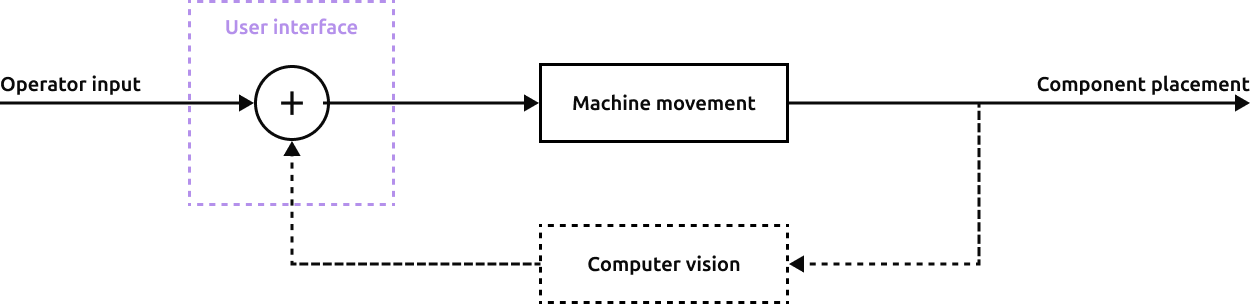
\includegraphics[width=0.9\textwidth]{Figures/block-diagram.png}
    \centering
    \caption{The prototype machine block diagram.}
    \label{fig:block-diagram}
\end{figure}

It is proposed that \ac{CV} `feedback' can be introduced to this open-loop control path to achieve enhanced machine performance \cite{AMAT2002473}.
This \ac{CV} would provide active alignment assistance to the human operator, offloading the burden of fine positioning to the machine.
In such an operating profile, the operator would be solely responsible for rough position identification.
Once component leads have been roughly associated with its corresponding component pads, active alignment assistance would correct any rotational error and perform final `wicking' of the component into place.

\subsubsection{Machine Modules}

To achieve the desired closed-loop feedback, a mechanical system that provides two real-time video feeds is devised.
One real-time video feed captures the \ac{PCB}'s pads, and another captures the picked component's leads.
This real-time video is fed to a \ac{CV} algorithm to identify the gantry translations and head rotations required to achieve wicking.

The experimental prototype comprises of three primary software modules and three supplementary electromechanical components, as diagrammed below in Figure~\ref{fig:architecture}.
\begin{figure}[hbtp]
    \includegraphics[width=0.9\textwidth]{Figures/architecture.png}
    \centering
    \caption{The prototype machine architecture.}
    \label{fig:architecture}
\end{figure}
The machine software comprises of the machine controller, the user interface, and the \ac{CV} routines.

The machine controller is written in Julia and is responsible for the control of the $x$-$y$ gantry and vacuum head, and communicates with these electromechanical components with standard RS-274 G-code.
The user interface displays the real-time video feeds of the \ac{PCB} and picked component to the human operator, and receives \& interprets their inputs through the third electromechanical component — the physical input device.
Real-time video streaming is achieved from the machine controller to the user interface by way of the \ac*{WebRTC} protocol.
The interface is implemented as a web browser application with Next.js in TypeScript, and implements low-latency full-duplex message passing with the machine controller through a WebSocket and \acfp*{protobuf}.
The \ac{CV} routines are implemented in a mixture of Julia and C, and is capable of identifying pad centroids for the controller and user interface to utilise.

A single \qty{4}{\giga\byte} Raspberry Pi 5 is used to run all three software modules, though the user interface may be served to any client browser that is networked to the Raspberry Pi.
The user interface may also be run on an operator's own device, provided there is a network connection to the Raspberry Pi such that the real-time \ac*{WebRTC} video feed and WebSocket connections can be established to the machine controller.

Further research and design discussion relating to the machine controller, low-latency communications, user interface, and \ac*{CV} follows below under respective headings.

\subsubsection{Mechanical Approach}\label{sec:Mechanical-Approach}

The focus on designing for \acl{CV} integration in the proposed machine imparted a number of critical design considerations that heavily influenced the mechanical approach that was undertaken.
Despite the indicative gantry repeatability of \qty{40}{\micro\metre} obtained in Section~\ref{sec:Repeatability} below, it was hypothesised that gantry and head repeatability was not a mechanical characteristic that could be relied upon for the developed prototype.
This dismissed any mechanical solution that relied on machine repeatability to maintain a representative prediction of component placement, such as the typical \ac{PnP} design featuring a fixed upwards-facing camera at a known absolute coordinate.

This resulted in the pursuit of a mechanical head design that could provide real-time video feeds of both \ac{PCB} and component without visual occlusions, as might be caused by the vacuum nozzle.
The guiding development aim for sufficient responsiveness with minimal loop delay to effectively integrate closed-loop active assistance led to the dismissal of any mechanical approach that would require extensive software vision correction of parallax error.
This narrowed the approach to a head design that provided a `matched' on-axis pair of video feeds, where the live component feed could be directly superimposed with the \ac{PCB} feed to present the operator with an accurate prediction of component placement.
This resulted in a `folding' head mechanism as shown in Appendix~\ref{apx:head-mechanism} that rotates the vacuum nozzle into the `downwards' position when picking or placing a component, then returning back to the `upwards' position to achieve real-time video from its two cameras.

Such a mechanical design enjoys the corollary advantage of being much less reliant on gantry repeatability.
If the human operator is continually presented with real-time video feeds of the picked component leads and target component pads, any mechanical error is trivially corrected by additional real-time human input.


\subsubsection{Computer Vision for Active Assistance}


Research suggests that computer vision can aid operators in achieving more precise spatial navigation with computer input devices, as demonstrated in teleoperation studies \cite{AMAT2002473}.
\Acl{CV} is employed in this project to facilitate active assistance in component placement by identifying features of interest on both the \ac{PCB} and the component being placed.
This is a departure from traditional \ac{PnP} machines, which rely on a priori knowledge of component and pad locations, typically encoded in Gerber files \cite{15543404}.
The project aims to devise a more organic and intuitive system that leverages real-time \ac{CV} to adapt to the operator's actions and the specific components being placed.

Initial considerations for \ac{CV}-driven placement focussed on identifying the centre of each component.
However, it was quickly realised that a more effective approach would be to match individual component leads with their corresponding \ac{PCB} pads.
This approach is not only more robust to variations in component orientation but also enables a more intuitive user interface, where the operator can select a single lead and the machine will automatically identify the matching pad and calculate the optimal rotation for placement.

A centroid finding algorithm was developed to identify the centre of each component pad.
This algorithm processes the real-time video feed captured from the downward-facing camera, identifying regions of interest that correspond to pad pixels.
The identified centroids are then used to guide the vacuum head towards the exact pad location.

In this context, a centroid represents the average $(x, y)$ coordinate of all pixels belonging to a particular feature \cite{10.1117/12.58623}, such as a component pad.
It can be thought of as the `centre of mass' of the feature; a single point that represents the location of the feature.

The centroid finding algorithm operates by first applying a threshold to the camera image, converting it to a binary representation where pixels are classified as either belonging to a feature or to the background.
This thresholding step leverages the colour difference between the metallic pads and the \ac{PCB}'s solder mask layer.
A connected component analysis \cite{edImageAnalysis} is then performed to identify groups of adjacent pixels that belong to the same feature.
For each identified connected component, the algorithm calculates the average $x$ and $y$ coordinates of all pixels bounded by that component, producing the centroid of the feature.
An example of this process is provided in Appendix~\ref{apx:centroids}.

Whilst the initial focus was targeted towards detecting the metallic pads of \acp{PCB}, the same principles can be applied to detect solder paste applied atop the pads.
This is essential for real-world functionality of such an active assistance mechanism, as \ac{SMT} components placed atop bare pads without solder paste applied first are not useful.
The challenge of solder paste detection lies in differentiating the paste from other features on the \ac{PCB}, such as silkscreen reference designators and solder mask.
Further research is required to explore different lighting techniques and image processing algorithms to achieve robust and accurate solder paste detection.

% ! ================================================== REPEATABILITY TESTING ==================================================

\subsection{Gantry Repeatability Testing}\label{sec:Repeatability}

It is established in Section~\ref{sec:Mechanical-Approach} that the pursued mechanical approach affords the prototype real-time \ac{PnP} machine with resilience against any repeatability issues with its $x$-$y$ gantry.
The designed operating profile of such a real-time machine features a critical advantage --- all gantry translations are performed relative to the current head position, and not with reference to an absolute datum.

Acknowledging the reduced importance of exceptional gantry repeatability in this application, an indicative repeatability test was conducted to profile the performance of the existing gantry frame.
An optical approach was undertaken, under the testing methodology of driving the gantry frame from a simple Julia machine controller with a pre-defined set of repeated G-code commands, and capturing thirty still images at each target position.
The captured still images are then composited to analyse any observed drift over many repeated gantry translations.
The measured drift is finally analysed to draw conclusions on any implications for placement accuracy or predictability.

A Raspberry Pi HQ \qty{12.3}{\megapixel} camera was used with a varifocal Arducam C-Mount Lens (model number \texttt{C20280M12}) as shown in Figure~\ref{fig:repeatability-rig}.
This varifocal lens and high-quality camera was used to permit a closer zoom with full optical focus, providing higher resolution images for greater measurement resolution.
Still images were captured with the \texttt{libcamera-still} command-line binary, with the set of option flags provided alongside the full Julia script in Program~\ref{lis:repeatability-script}.

The thirty still images captured at each point were composited with the script provided in Program~\ref{lis:repeatability-composite}, an example output from which is shown below in Figure~\ref{fig:repeatability-composite}.
The hue of each individual image in the rainbow composite represents the repetition index, i.e. red indicates the first capture, and white indicates the last capture.
These results were encouraging, despite the clearly observable variation in gantry position.
It is important to note that neither the gantry nor camera were rigidly mounted in this indicative repeatability test due to limited mounting hardware, so potential error resulting from movement of the machine frame or camera mount is to be expected.
It is indeed observed through the resultant rainbow that the gantry drift exhibits in a constant direction, and the gantry position is not randomly distributed about some central mean.
This suggests that the error does result from movement of the machine frame or the camera mount, rather than any error inherent in the gantry's belts or steppers.
\begin{figure}[hbtp]
    \includegraphics[width=0.475\textwidth]{Figures/repeatability-raw.png}
    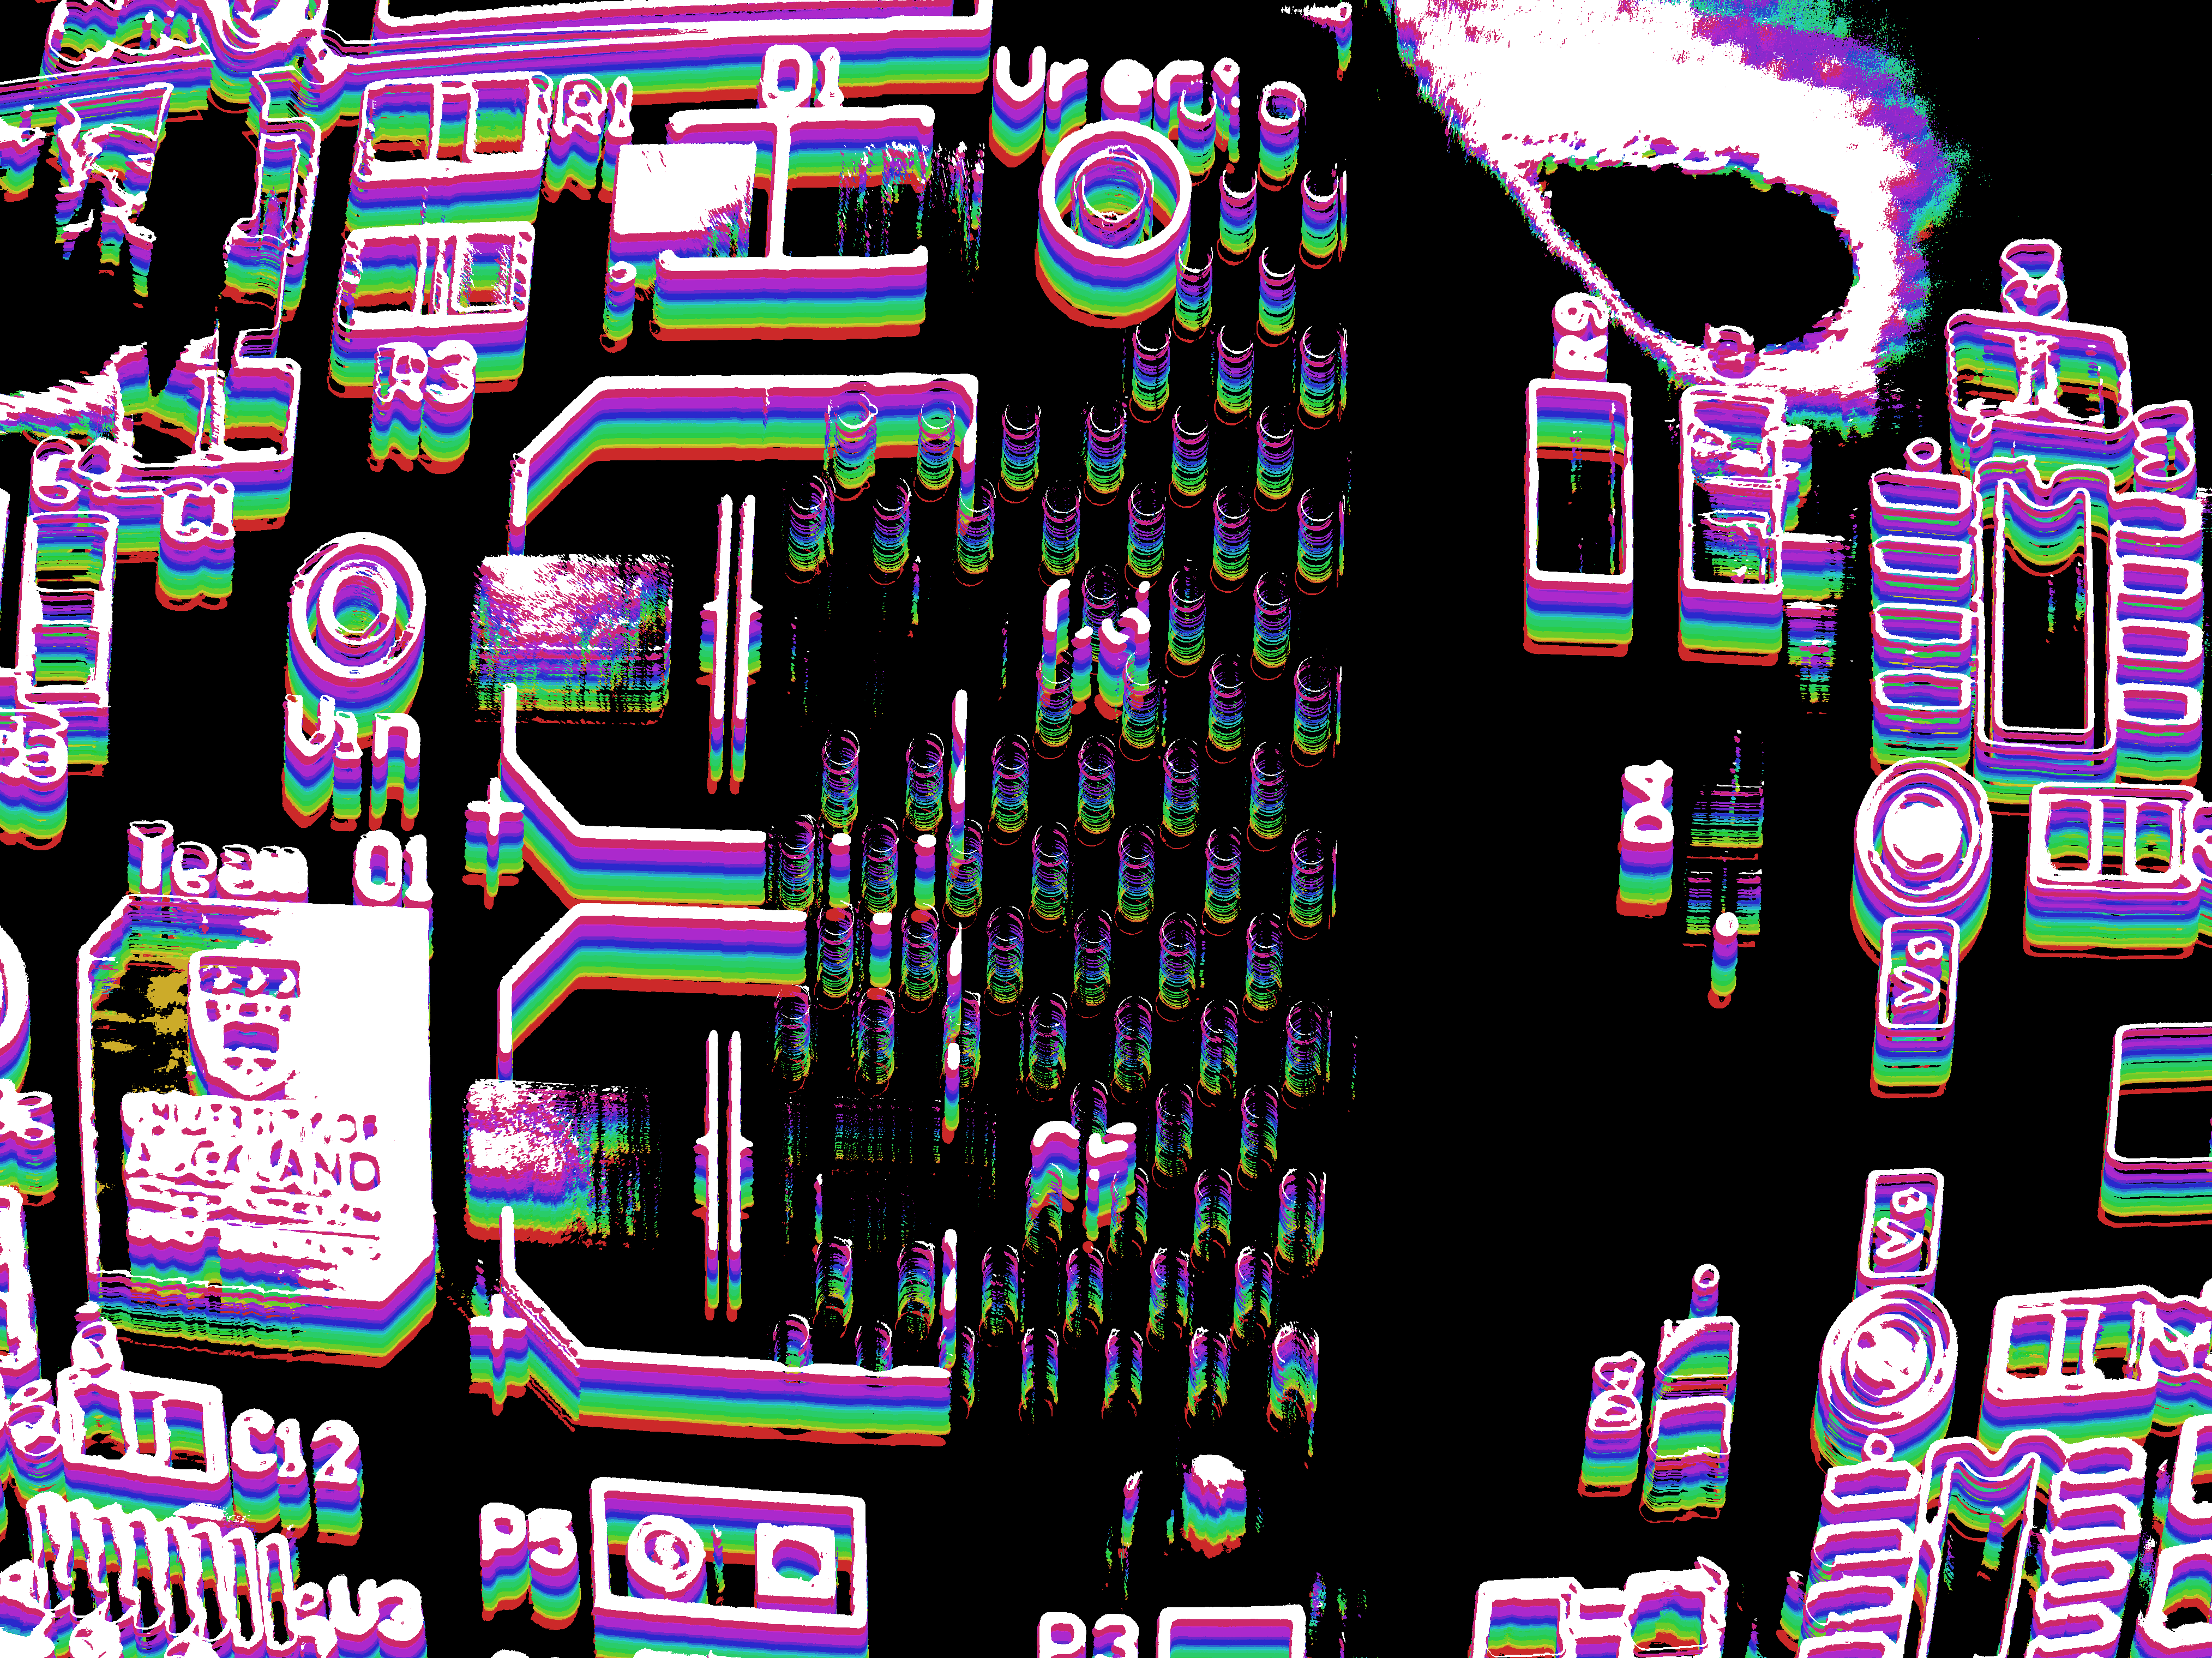
\includegraphics[width=0.475\textwidth]{Figures/repeatability-colour.png}
    \centering
    \caption{The raw and composited still images at a selected point.}
    \label{fig:repeatability-composite}
\end{figure}

It is known from the Gerber production file of the pictured test \ac{PCB} that each photographed via is of \qty{0.5}{\milli\metre} hole diameter, such that a drift of \qty{1.18}{\milli\metre} is measured in Figure~\ref{fig:repeatability-annotated} over thirty repetitions.
Dividing by the number of repetitions, an indicative repeatability of \qty{40}{\micro\metre} is produced under this rudimentary test methodology --- i.e. translating to a particular absolute coordinate, moving through nine other points, then moving back to the same absolute coordinate within \qty{40}{\micro\metre}.
This repeatability would not suffice for full open-loop, pre-programmed machine operation, but is expected to be suitable for the devised real-time, human-in-the-loop control method.
This result suggests that the $x$-$y$ gantry is unlikely to be the limiting component of the prototype machine when considering minimum component size --- rather, this constraint is likely to be defined by the vacuum nozzle diameter.
\begin{figure}[hbtp]
    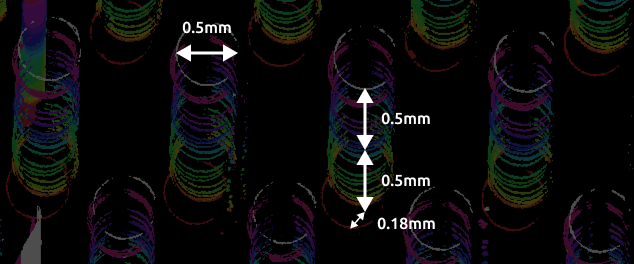
\includegraphics[width=0.8\textwidth]{Figures/repeatability-annotated.png}
    \centering
    \caption{The drift of \qty{1.18}{\milli\metre} observed over thirty repetitions.}
    \label{fig:repeatability-annotated}
\end{figure}

% - We then re-ran a similar repeatability test after Sam had re-built the gantry and attached the new head mechanism, to see changes (if any).
% - This was done with the CM3 that is actually going to be used on the head.
% - We removed the homing operation, as the machine should never need to home whilst in operation — which removes one potential source of error.
% This is because the gantry firmware uses the limit switches at (x=0, y=0) to zero its internal position state.
% Consequently, any variability in the electro-mechanical limit switch homing process (mechanical contact, electrical signal change, firmware sample and detection) will introduce some offset in the zero position.
% This offset would directly transfer into the absolute coordinates specified in the repeatability tests.

% ! ================================================== VIDEO STREAMING ==================================================

\subsection{Video Streaming}

\subsubsection{Initial Exploration}

A fundamental requirement of our real-time prototype machine lies in the need for low-latency video from both cameras by both the human operator through the user interface and the machine's \ac{CV} routines.
This video streaming implementation must be sufficiently low-latency to maximise the responsiveness \cite{Z.2022} of the open-loop machine.

Initial network streaming testing of the video feed from a Raspberry Pi and an attached camera exhibited over \qty{2}{\second} of latency with \ac{TCP} as produced by Program~\ref{lis:video-tcp}, which was considered wholly inadequate.
This latency was measured by pointing the camera lens at a laptop screen, then measuring the time taken after changing a portion of the laptop screen from black to white before observing that same visual change in the received video feed.

UDP streaming was also tested, but significantly longer frame delay and poorer video quality was found.
Although \ac{TCP} streaming was considered too slow for real-time processing, the \ac{UDP} video stream contained many visual artefacts that corrupted the received image.
Continued experimentation with \ac{TCP} streaming configuration produced Program~\ref{lis:video-tcp}, though this still delivered unsatisfactory results.

Further research suggested that \ac{RTSP} could be used to achieve latency in the order of \qty{1}{\second} \cite{codecalamityRaspberryStreaming}, however the test stream as provided in Program~\ref{lis:video-rtsp} failed to work.

A comparison of various video streaming protocols and their latencies with a Raspberry Pi 5 was found that supported the observed \ac{TCP}, \ac{UDP}, and \ac{RTSP} results \cite{mediumRaspberryVideo}, which also identified the open-source MediaMTX software as a functional streaming solution capable of \qty{200}{\milli\second} latency.
MediaMTX is a real-time media server that routes video and audio streams from input to output with many supported streaming protocols, including \ac{RTSP} and \ac{WebRTC} \cite{mediamtx}.
Although the MediaMTX \ac{RTSP} output was successfully streamed to the test laptop, a poor \qty{6}{\second} latency was observed.

\subsubsection{\acf*{WebRTC} Protocol}\label{sec:WebRTC-Video-Streaming}

Testing MediaMTX with \ac{RTSP} input and \ac{WebRTC} output, a latency of \qty{130}{\milli\second} was achieved whilst running the repeatability routine as shown in Figure~\ref{fig:latency-rig}.
This was a $1280\times720$ pixel stream at 30 frames per second, with virtually zero latency when viewed by human eye.
\ac{WebRTC} is an open-source project that provides web browsers and mobile applications with real-time communication capabilities via simple \acp{API} \cite{webrtc,mozillaWebRTCAPIs}.
It enables peer-to-peer audio, video, and data communication.

% ? A nice figure

The resultant low-latency video streaming solution is therefore a MediaMTX real-time media server that is used to stream real-time video from the Raspberry Pi's cameras to the user interface over the \ac{WebRTC} protocol.
The individual video streams are first read by the Julia \ac{CV} routine from the camera sensors with the \texttt{rpicam-vid} command-line binary, which is distributed as part of Raspberry Pi OS.
The \ac{CV} routine then composites the two feeds together to produce the final real-time video feed showing predicted component alignment as shown in Figure~\ref{fig:component-aligning}.
This feed is then written to \texttt{ffmpeg}, which transcodes the video from its raw \texttt{YUV 4:2:0} format into \texttt{H.264} and streams the transcoded feed to MediaMTX via \ac{RTSP}.
A simplified MediaMTX \texttt{runOnInit} script to stream real-time video from a single camera is provided below in Program~\ref{lis:video-mediamtx}.
\begin{figure}[hbtp]
    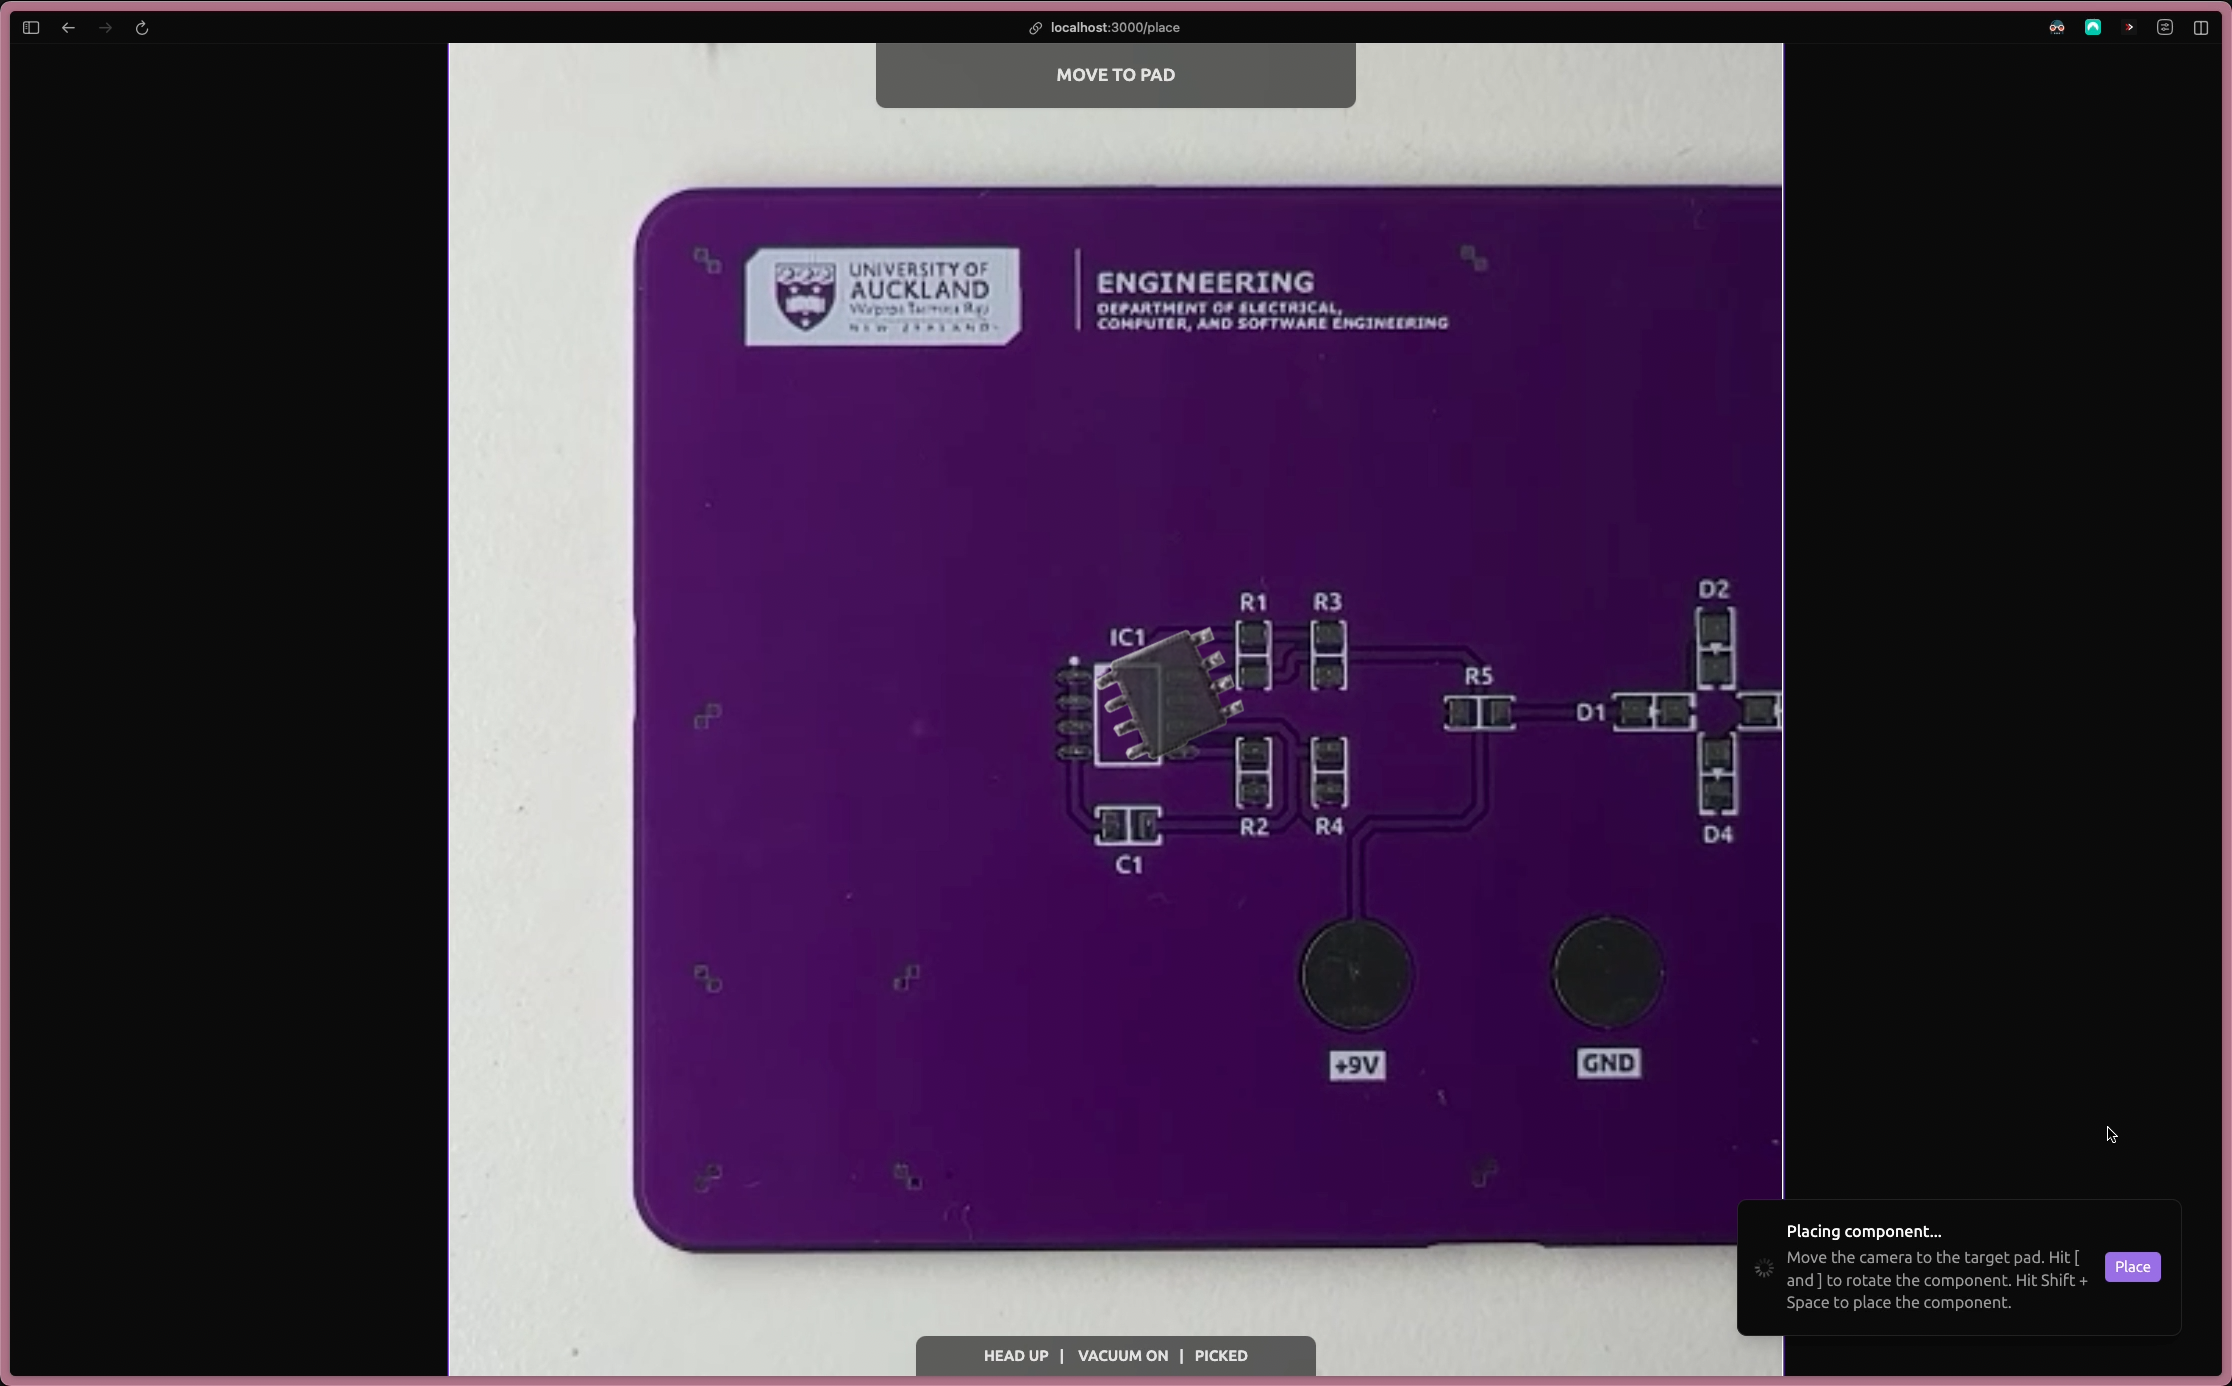
\includegraphics[width=0.8\textwidth]{Figures/component-aligning.png}
    \centering
    \caption{Real-time composite video feed showing the picked component and \ac{PCB} pads.}
    \label{fig:component-aligning}
\end{figure}

Once the \texttt{H.264} video is streamed into MediaMTX, it can then be read from the server via any of its supported protocols and variants.
The user interface client reads the stream via the \ac{WHEP} variant of the \ac{WebRTC} protocol before displaying it to the operator in a \texttt{<video>} \ac{HTML} element.
The egress of the video stream is implemented with \texttt{Evevinn/webrtc-player}, an open-source library to play \ac{WebRTC} streams in client browsers \cite{webrtc-player}.

Of particular further interest was the support within the \ac{WebRTC} protocol for data channels to exchange arbitrary messages alongside the streamed video \cite{13807501}.
Just as real-time, low-latency video is imperative to the functionality of the hybrid \acl{PnP} prototype, so too is data exchange between the interface and the machine controller.
\ac{WebRTC} data channels were identified as a potentially convenient solution to this need, which is discussed further in Section~\ref{sec:Controller-Interface-Messages}.

% ! ================================================== MESSAGE PASSING ==================================================

\subsection{Message Passing}

The same desire for low-latency video applies to the data exchange between machine modules.
This requires deliberate, well-engineered message design for time- and space-efficiency.

\subsubsection{Controller to Gantry}\label{sec:Controller-Interface-Messages}

The machine controller communicates with the gantry and vacuum head using the industry standard RS-274 G-code protocol, transmitted over a \texttt{115200}-baud USB serial port.
G-code is a numerical control programming language widely used for controlling automated machine tools \cite{02683768}, and provides a simple method of specifying movements and actions.

Initially, a complete re-implementation of the gantry firmware was considered to optimise for minimal message length and transmission time.
This was motivated by the desire to maximise machine responsiveness by minimising the number of bits transmitted for each command
However, it was ultimately decided to leverage the existing \texttt{Grbl} open-source G-code interpreter for its maturity, robust feature set, and extensive documentation \cite{grbl}.
This decision allowed focus to be placed on higher-level aspects of the project, such as the development of the shared control scheme and the user interface.


\subsubsection{Controller to Interface}\label{sec:Controller-Interface}

A persistent, full-duplex connection is imperative between the machine controller and the user interface to facilitate real-time data exchange.

\paragraph{Messaging Channel}
The \ac{WebRTC} streaming protocol used for real-time video does feature support for data channels, as discussed in Section~\ref{sec:WebRTC-Video-Streaming}.
Initial research profiled the feasibility of this solution, which revealed that this feature of \ac{WebRTC} was not suitable for the prototype machine.
It was discovered that support for data channels between broadcaster and player was once supported by the selected \texttt{Eyevinn/webrtc-player} \ac{WebRTC} client \cite{githubDatachannelSupport}, but this support has been subsequently removed \cite{githubFeatRemove}.

Further, it was discovered that the MediaMTX media server used to stream video to the interface via \ac{WebRTC} does not support for custom data channels \cite{githubTransmittingData,githubDataChannel}.
Additional concerns arose regarding the complexity of implementing a \ac{WebRTC} server in Julia, given the limited availability of existing tooling and libraries.

Consequently, a standard WebSocket connection was chosen for its relative implementation simplicity, maturity, and widespread support \cite{MitrovicNikola2023IATO,mozillaWebSocketWebSockets}.
The usage of a separate data exchange mechanism was in fact advantageous due to the resultant decoupling of message passing from video streaming, achieving a separation of concerns.
WebSockets provide a real-time, low-latency, full-duplex communication channel \cite{6197172,OgundeyiK.E.2019Wirt} that is well-suited for the long-lived, instant messaging required between the user interface and the machine controller.

To profile the suitability of this WebSocket messaging protocol towards the development of a responsive \ac{PnP} prototype, a simple test was devised to verify the speed and functionality of this duplex connection.
The Julia machine controller was updated to provide mock responses to the user interface upon receiving an operator click input.
A simple routine was written to incrementally `step' a received click delta back towards the centre of the screen, where each incremental step would be notified back to the user interface.
This routine is provided in Program~\ref{lis:socket-mock-server}.

The user interface was updated to display these simulated machine steps by updating the position of a \acl*{HUD} target indicator, where this target indicator would initially reflect the input click position before incrementally stepping to the viewport centre as response messages were received from the machine controller.
With this setup, the speed and responsiveness of the data channel could be easy visualised through the speed at which the target indicator returned to the centre of the screen.
This simple test was highly encouraging, as even many tens of these incremental `step' messages could be received and processed by the interface near instantaneously --- and considerably faster than a human operator could present inputs to, or process outputs from, the interface.

\paragraph{Normalised Coordinate Space}
As also discussed in Section~\ref{sec:User-Interface}, the operator's click coordinates must be normalised with respect to the client \ac*{DOM} viewport width.
The viewport represents the size of the user interface's browser window \cite{mozillaViewportConcepts}, which presents itself as an unknown variable about which the machine controller has no awareness.
If the raw $(x, y)$ click coordinate in viewport pixels as emitted by the JavaScript mouse \texttt{onclick} event were to be transmitted to the controller, a click at the far right-edge in a full-screen browser window would result in twice the gantry translation distance than a half-width browser window.

A naïve solution might be to map every client click coordinate into the streamed video dimensions, i.e. a click on the far-right edge of a $1920\times1080$ pixels video would be mapped to an abscissa of \qty{1080}{\px} regardless of viewport size.
This approach requires an assumption that the video dimensions will not be scaled at runtime, or that the machine controller maintains knowledge of the streamed video dimensions at all instants of time.
A third requisite assumption exists that the machine controller knows the relationship between camera pixels and real machine bed distance units.
This third assumption is not trivial, as the streamed video \ac{FoV} is largely independent of video resolution --- camera pixels are independent of distance units.

The solution taken is not to map into, but to normalise click coordinates with respect to video height and width such that each coordinate exists within the range $[0, 1]$.
This reliance on floating-point numbers is undesirable from the lens of time- and space-efficiency however, such that the normalised values are then scaled into a \qty{16}{\bit} integral type to implement a form of fixed-point number.

The difficulty here lies in the number of distinct measures of 'distance', many of which are not related by a constant scaling factor.
Many of the relationships between these measures are dependent on external variables including workbed \& head height, camera \ac{FoV}, and the continually-iterating mechanical head and gantry implementation.
These measures are the client viewport pixels, camera sensor pixels, and streamed video pixels (\unit{\px}); machine stepper step count (unitless); and workbed distance (\unit{\milli\metre}).

The resultant coordinate space for data exchanged between the machine controller and user interface can be described as a relative Cartesian coordinate space measured against the position of the head.
The space is centred at $(0, 0)$.
This origin $O$ represents the current position of the head, and ideally corresponds to a browser viewport position of $(50\%, 50\%)$.
The axes are unitless; with values representing a ratio of $\unit{\px} / \unit{\px}$.
Both axes are of $2^{16}=65,536$ total range.
Each axis is maximimally negative at $-32,768$ and maximally positive at $32,767$.

Following this normalisation process, the deltas exchanged between the two software modules are agnostic of such runtime variables as the client viewport and streamed video size.
The burden is thus left to the receiving module to map the dimensionless ratio into the real unit of interest, whether real camera pixels, machine steps, real distance, or viewport pixels.
A calibration routine has been developed as detailed in Section~\ref{sec:Calibration} that can be run from the user interface when such mechanical variables as workbed height or machine stepper gear ratio are changed.
This calibration routine will correct the conversion factors within the Julia machine controller without requiring any changes to source code.

\paragraph{Message Format}
Careful design was also undertaken towards specifying the messaging format between the machine controller and the user interface, with a number of iterations being performed.
The initial message specification was designed as a \texttt{Uint8} byte stream, where the first byte of each message represented a `tag' that described the message type.
This `tag' was used by the receiving module as a codeword to distinguish between messages and correctly parse and handle each message type.
All subsequent bytes in the stream are an optional arbitrary payload that is defined by each message type.
TypeScript language semantics were used to explicitly define the payload format that corresponded to each message tag, preventing system misbehaviour following from malformed messages.
Similarly, all receiving modules implemented full validation on received messages, performing no operation if a misshapen message was received.

A \ac{MWE} was then developed of low-latency communiction between the user interface and machine controller, implementing the devised message specification and coordinate space normalisation.
This \ac{MWE} is detailed in Appendix~\ref{apx:websocket-testing}.
A snapshot of this \ac{MWE} is shown in Figure~\ref{fig:latency-message} below.
\begin{figure}[hbtp]
    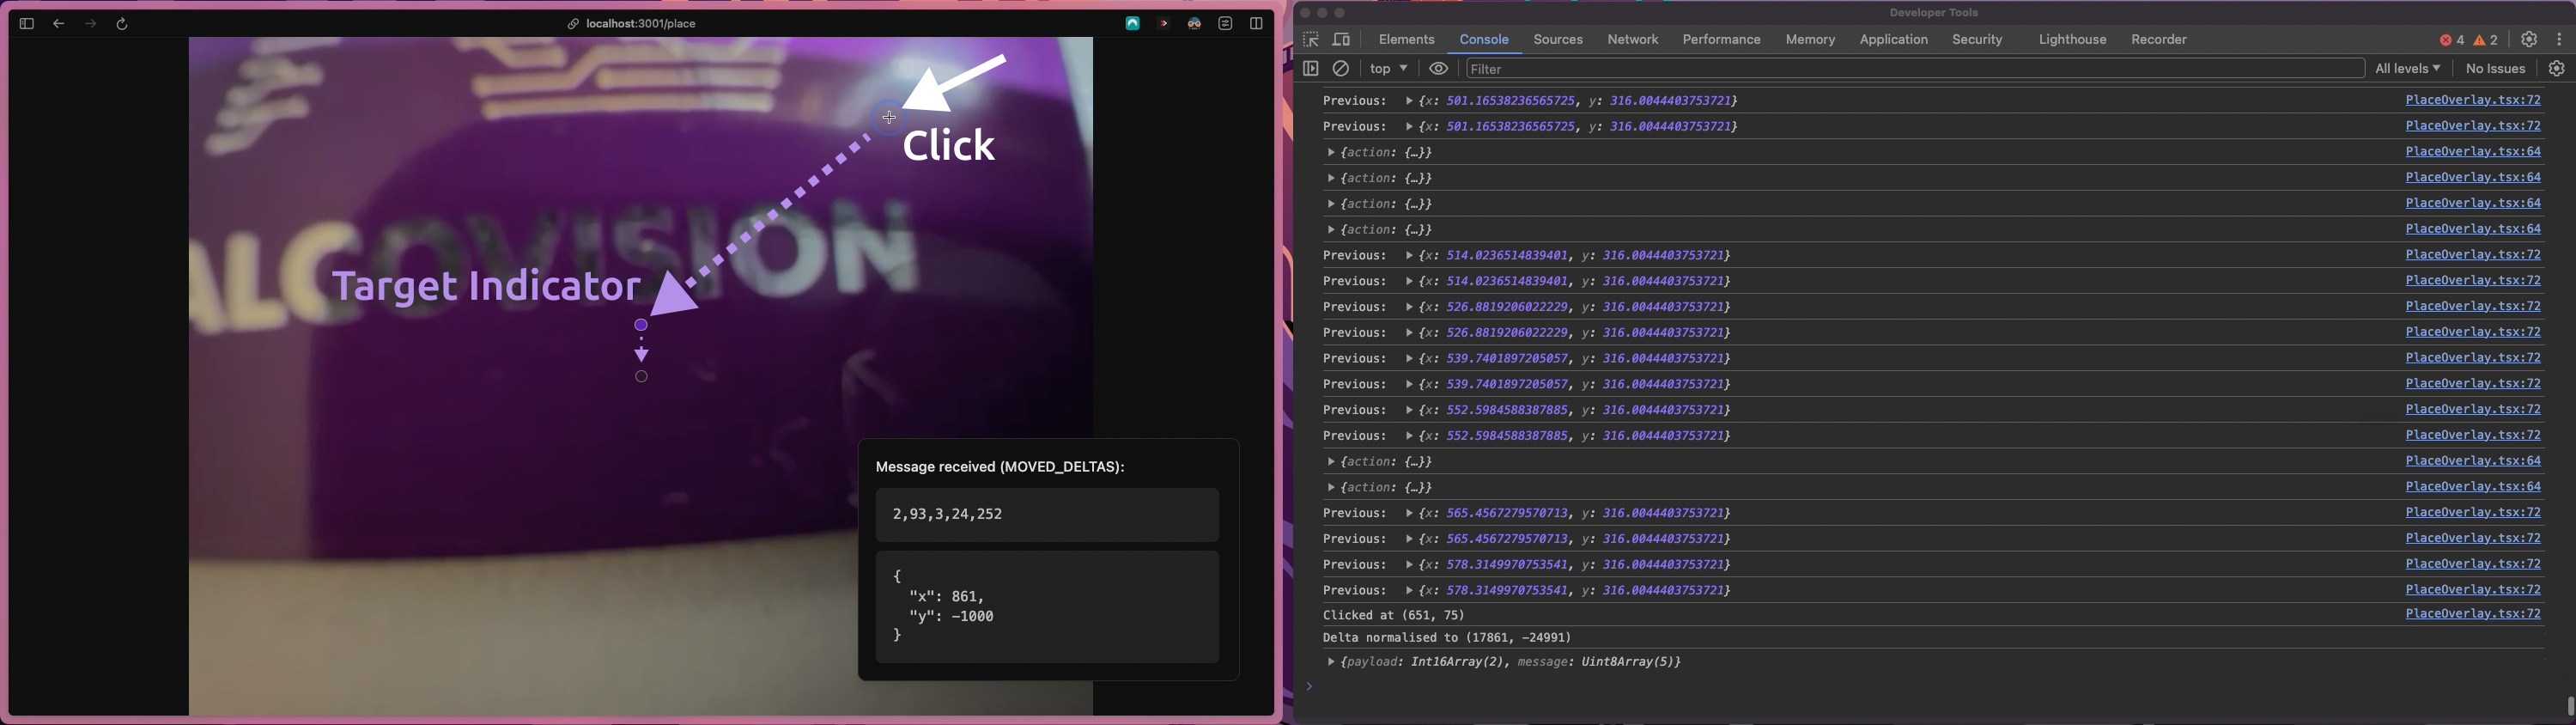
\includegraphics[width=\textwidth]{Figures/latency-message.png}
    \centering
    \caption{A snapshot showing the target indicator in motion towards $(0, 0)$.}
    \label{fig:latency-message}
\end{figure}


\paragraph{Protocol Buffers}
Literature was further investigated following the implementation of this simple messaging specification.
It was anticipated that the application's demands would come to necessitate more structured data exchange, for which the simple messaging specification could not be trivially extended.
For instance, the basic messaging format was not designed with consideration for arbitrary-length repeated data, as is required for array types.
A possible extension to the specification to support array types might be the inclusion of an additional leading byte representing the length of the data, though this solution would not support arrays beyond a length of $2^8 = 256$.
Another solution might be to simply transmit the array as the payload byte stream, and place the expectation on the receiving module to delineate between each element through clear definition of each array's element data type such that the number of bytes per element is known.

It was discovered that \acp{protobuf} are designed for exactly this purpose \cite{5982183}, and are significantly more efficient that other structured formats like \ac{JSON} or \ac{XML} \cite{6784954,8337257}.
\Aclp{protobuf} were subsequently implemented for all data serialisation and exchange between the machine controller and user interface.

Although these \acp{protobuf} replaced the previous message specification, heavy inspiration towards the design of each message was carried through.
Each message retains a \texttt{tag} field; a \qty{1}{\byte} enumeration that represents the message type.
The \texttt{Message} \ac{protobuf} message contains only a single other field, the \texttt{payload}.
This payload is defined as a \texttt{oneof} \ac{protobuf} field, which behaves simiarly to a C \texttt{union}
in that at most one payload field may be set at any given time, as all fields in a \texttt{oneof} occupy the same memory \cite{protobufLanguageGuide}.
As with the preceding message specification, each \texttt{tag} is associated with an expected payload.
This is a contract that is understood by both the transmitting and the receiving module.
The receiver validates that the received message payload matches the expected type for the given \texttt{tag}, ensuring data integrity and preventing errors caused by malformed messages.
The \texttt{pnp.proto} language definition file is provided at Program~\ref{lis:pnp-proto}.

The adoption of \acp{protobuf} results in minor penalties to the space- and time-efficiency of data exchange when compared against the previous specification due to additional housekeeping `varint keys' \cite{protobufEncoding}.
However, these losses are deemed acceptable when acknowledging \acl{protobuf} support for \texttt{repeated}/array-type fields, optional fields, default values, and more \cite{protobufLanguageGuide}.
Importantly, \Aclp{protobuf} also feature `variable-width integers', encoding smaller unsigned integers into only as many bytes as is necessary \cite{5982183,protobufEncodingVarints}.
This is a core feature of \acp{protobuf}, and affords space savings whenever possible --- provided messages are carefully designed with data types that support variable-width encoding.

The combination of WebSockets and \aclp{protobuf} provides a robust and efficient solution for real-time communication between the interface and the controller, ensuring low-latency and reliable data exchange in a space-efficient binary format.

\subsubsection{Machine Controller Calibration}\label{sec:Calibration}

A calibration routine was developed for the operator to fine-tune the conversion factors used by the machine controller and improve placement accuracy.
This routine is accessed from the user interface, and is necessary whenever the relationship between camera pixels and real machine bed distance units is changed.
This could be, for example, as a result of adjusting the height of the machine bed, or if the stepper motors' gear ratio is changed.

The key principle of the prototype machine's calibration is that all conversions and corrections pertaining to the physical mechanics are performed by the Julia machine controller.
The Julia machine controller behaves as a translation layer, or adapter, between the operator inputs to the user interface and the physical $x$-$y$ gantry or vacuum head.
The user interface is decoupled from any knowledge of the physical layer, and is only responsible accepting user input in viewport coordinates then normalising this to the machine's standard coordinate space.
It is the machine controller that is responsible for translating the normalised numeric data from the user interface into the real-distance units for the gantry.

An initial draft of a calibration algorithm was produced, that guided the operator to click on a series of grid squares in order to calibrate the horizontal and vertical axes independently.
This initial calibration algorithm is provided in Appendix~\ref{apx:calibration}.

It was quickly realised that this calibration routine is not robust, as calibrating each axis independently could result in significant errors if the operator reports position error in the complementary axis.
Consider a case where the operator attempts to calibrate the machine's $x$ axis.
Inherent imprecision in mouse input may result in a $y$-delta of $1$ to be messaged to the controller, even if the operator believes that they clicked perfectly to the right.
If a $y$-delta of $2$ caused by the same imprecision is reported to the controller in the \texttt{CALIBRATE\_DELTAS} message, the controller will erroneously recompute its $y$ conversion factor to be half of its previous value --- resulting in significant error.

This could be solved by enforcing that the operator first calibrates $x$, then calibrates $y$, and by ignoring all deltas in the complementary axis.
However, this introduces implementation complexity and convolutes the calibration process.
If the distance error between the expected and actual positions is small, then any error in the operator's corrective input will contribute a larger relative contribution to any changes in the calibration factor.

The algorithm was revised to address this issue, by instructing the operator to select calibration points that lie diagonally from each other.
The calibration patterns were also revised with the removal of the `fine' calibration scale, as it was found that user input imprecision influenced the calibration factors far too significantly.
It was also discovered through experimentation that the checkerboard pattern was far too difficult to use, as it was difficult to track any particular grid corner as the machine gantry translated.

The checkerboard pattern was therefore replaced with distinct and variably-spaced fiducials, as designed on the custom calibration boards shown in Figure~\ref{fig:calibration-board}.
These fiducials are intentionally designed differently to standard \ac{PCB} fiducials, as the circular pad does not clearly present a single defined point at which to click.
Finally, these test boards implement an operational amplifier oscillator circuit that flashes an array of \acp{LED} when excited by a \qty{9}{\volt} battery, as per the schematic shown in Figure~\ref{fig:calibration-board-schematic}.
This is a simple circuit that comprises of an \texttt{SO-8} \ac{SMT} \acf{IC}, a number of \texttt{0805} passive \ac{SMT} components, and some \ac{SMT} \acp{LED}, allowing for basic benchmarking of the developed prototype.
\begin{figure}[hbtp]
    
\includegraphics[width=0.495\textwidth]{Figures/calibration-board-top.png}
    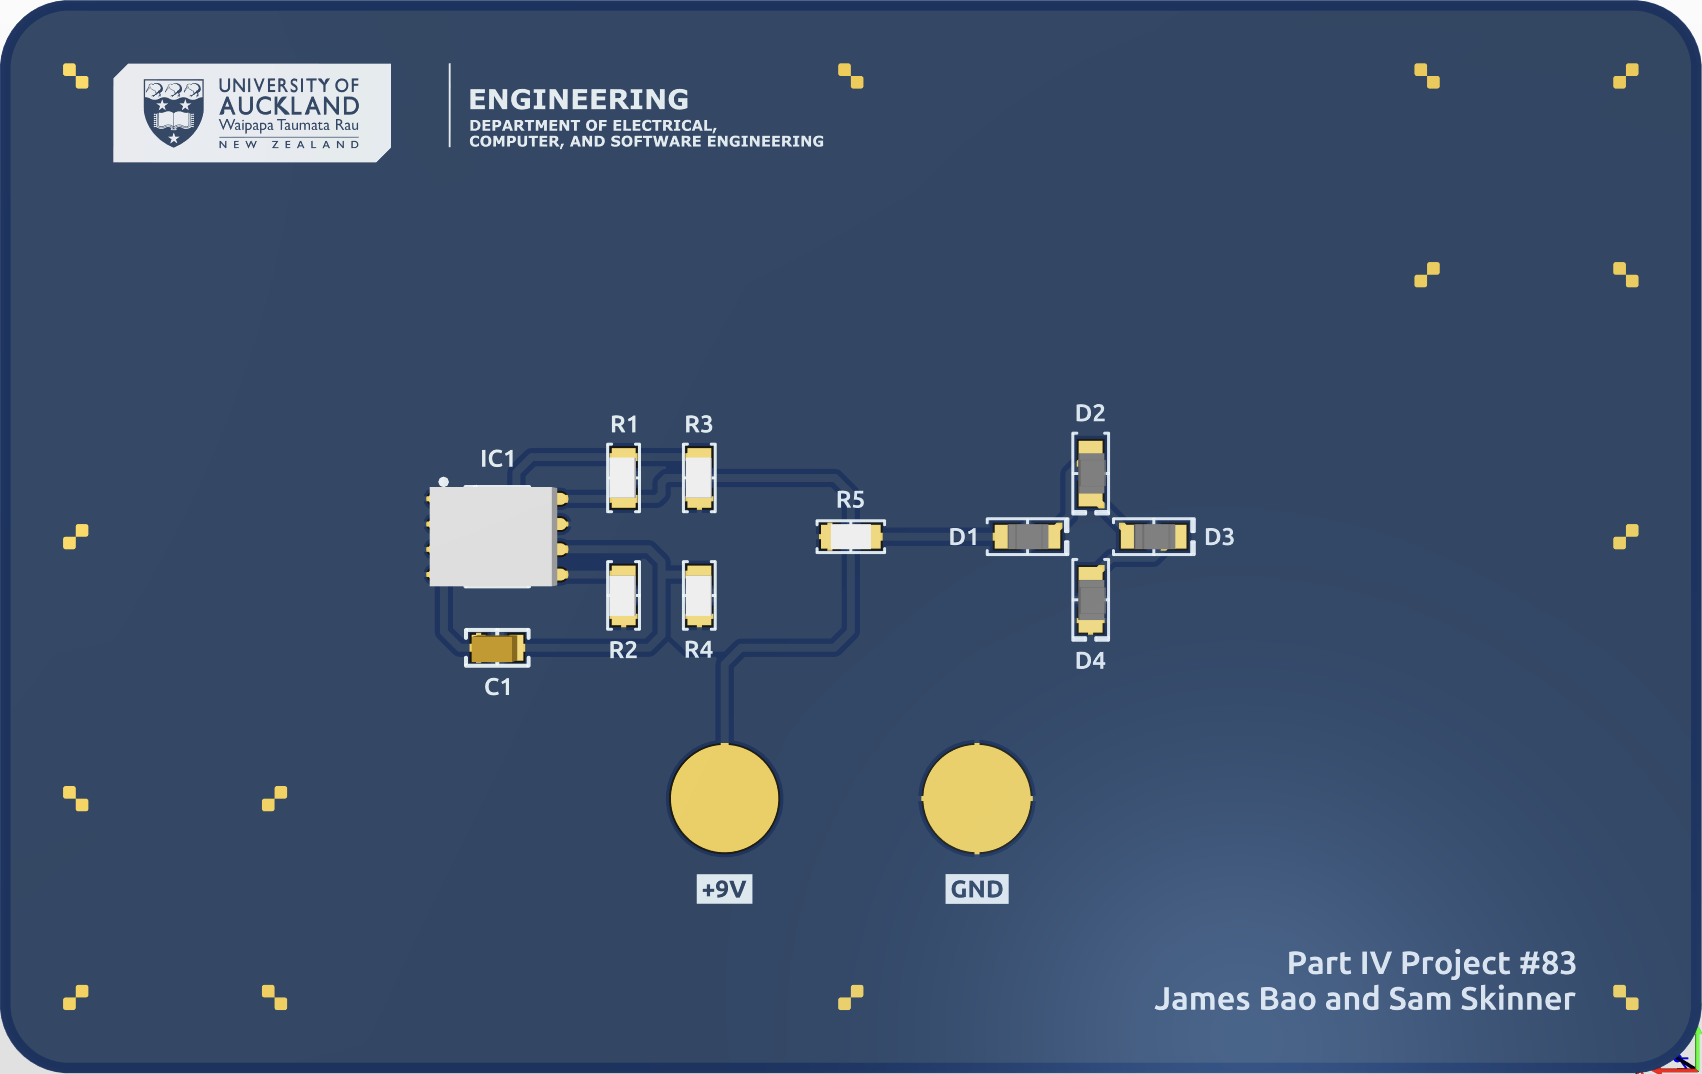
\includegraphics[width=0.495\textwidth]{Figures/calibration-board-bottom.png}
    \centering
    \caption{The test and calibration board designed for the prototype \ac{PnP} machine.}
    \label{fig:calibration-board}
\end{figure}

The final implementation of the calibration routine is as follows:

\begin{enumerate}
    \item Place a calibration board onto the workbed.
          The board does not need to be aligned with the axes, nor does the nozzle need to be moved directly atop a fiducial.
    \item Click on a diagonal calibration fiducial.
          The interface transmits a \texttt{TARGET\_DELTAS} message to the controller.
    \item The machine controller receives the \texttt{TARGET\_DELTAS} message and translates the gantry by the specified number of deltas, based on its current $x$ and $y$ calibrations.
    \item Click on the new viewport coordinate of the previously-clicked calibration fiducial, or hit space if it is exactly correct beneath the nozzle.
          The interface transmits a \texttt{CALIBRATE\_DELTAS} message to the controller.
    \item The machine controller uses the \texttt{CALIBRATE\_DELTAS} payload to re-compute its scalar factors as per Equation~\eqref{eq:calibration}.
    \item Repeat until satisfied with machine calibration.
\end{enumerate}

The \texttt{CALIBRATE\_DELTAS} payload contains the previously-transmitted target deltas $\Delta_\text{t}$, in addition to the deltas $\Delta_\text{r}$ of the point to which the fiducial actually travelled.
The \acl{protobuf} strucutre for this \texttt{Calibration} message is provided in Program~\ref{lis:pnp-proto}.
These two deltas are used by the machine controller to re-compute its conversion factors $(c_\text{x}, c_\text{y})$ through Equation~\eqref{eq:calibration} as derived in Appendix~\ref{apx:calibration-derivation}.

The corrected calibration factor $c'$ is computed by
\begin{equation}
    c' = c \times ((\Delta_\text{t} - \Delta_\text{r}) / \Delta_\text{t})
    \label{eq:calibration}
\end{equation}

This calibration routine allows the operator to accurately calibrate the machine controller to resolve any changes in physical mechanical machine parameters without requiring changes to machine source code, ensuring precise and repeatable component placement.

% ! ================================================== USER INTERFACE ==================================================

\subsection{User Interface}\label{sec:User-Interface}

The user interface is a crucial component of the semi-automated \ac{PnP} machine, and serves as the primary means of interaction between the human operator and the machine controller.
It is responsible for presenting the real-time video feeds from the cameras, displaying relevant information about the machine's state and operation, and accepting and interpreting the operator's input.
The design of the user interface is paramount to the success of the project, as it must be both efficient and intuitive to use --- promoting a state of flow without hindering the operator with complex or cumbersome operations.

A number of user experience considerations have been made to improve the prototype's user interface.
A loading bar is displayed whilst establishing the \ac{WebRTC} video connection to provide feedback to the operator and prevent premature interaction.
Graceful error handling is also implemented to address \ac{WebRTC} video errors, displaying an error message to the operator and suggesting possible solutions.


\subsubsection{Technical Implementation}\label{sec:User-Interface-Technical}

The user interface is implemented as a web application, leveraging the ubiquity and flexibility of modern web browsers.
This approach enables portability, allowing the operator to control the machine from any device with a web browser and network connection to the machine.
This eliminates the need for a dedicated monitor attached to the \ac{PnP} machine.

% The choice of a web application is further justified by the ease of development afforded by the mature ecosystem of web development technologies and tools that provide a rich selection of libraries, frameworks, and resources for rapid prototyping and development.
% This rapid iteration and refinement of the user interface has been enabled by these considerations.
% Another key advantage of this approach is its ability to leverage the computational power of the operator's device, providing scope to offload computationally intensive processing from the resource-constrained Raspberry Pi.

The initial design of the user interface explored using the \ac{HTML} \texttt{<canvas>} \ac{API} for its flexibility in drawing graphics and handling user input \cite{10109201}.
This approach would have enabled the implementation of a \acf{ZUI} as identified in literature \cite{doi:10.1080/0144929X.2011.586724}, where the operator could pan and zoom around a high-resolution image of the \ac{PCB}.
This idea was further explored by considering the use of \ac{WebGL}, which would have enabled hardware-accelerated graphics rendering to improve performance and responsiveness \cite{mozillaWebGLGraphics}.

A tile-based map interface composed of still images at various zoom levels was also considered to reduce bandwidth requirements.
This approach would have involved capturing a high-resolution image of the entire \ac{PCB} at the start, then capturing smaller, more-zoomed tiles that could be loaded on demand as the operator navigated around the board.
These concepts of a \ac{ZUI} and feed-forward control is discussed further in Section~\ref{sec:Future-Enhancements}.

Upon further research into the \texttt{<canvas>} element, it was ultimately deemed to be poorly documented \cite{10109201} and less intuitive for development.
The event handling model for \texttt{<canvas>} is less intuitive than that of standard \ac{HTML} \ac{DOM} elements, requiring more complex code to handle user interactions \cite{canvasEvents}.
The final implementation of the user interface therefore opted for a simpler approach using standard \ac{HTML} elements like \texttt{<div>}s for layout and interaction, with provision for further investigation into \texttt{<canvas>} and \ac{WebGL} if advanced graphics were needed in future.

A \texttt{<div>} overlay \acs{HUD} is positioned directly atop the \texttt{<video>} element that displays the real-time \ac{WebRTC} video feed.
The overlay dynamically resizes to match the dimensions of the streamed video.
A crosshair cursor style is applied to the mouse pointer within the overlay to provide the operator with visual feedback, indicating the exact location on the \ac{PCB} that will be targeted by the machine.
The operator's mouse click viewport coordinates are normalised into an \texttt{Int16} coordinate space as detailed in Section~\ref{sec:Controller-Interface}.

\subsubsection{Design Considerations for Flow}

A primary focus of the user interface design was on achieving a state of flow for the operator, as defined by \cite{csikszentmihalyi2000beyond}.
To induce flow, the interface needed to provide clear goals, immediate feedback, and a balance between challenge and skill.
The design of the user interface was further guided by the principles of shared control, aiming to create a system that seamlessly blends human input with machine assistance \cite{Dragan2013}.

\paragraph{Joystick and Shared Control}
Initial explorations considered a joystick and an encoder knob as the primary input devices for controlling the machine.
The joystick would have allowed for intuitive control over the vacuum head's position, offering a familiar and proportional method of specifying machine velocities in the $x$ and $y$ directions.
The encoder knob would have provided a mechanism for adjusting the angular rotation of the picked component around the $z$-axis, allowing for precise rotational control.
This approach was particularly appealing due to its resemblance to common video game control schemes, which are known for their intuitiveness and ability to promote a state of flow \cite{doi:10.1177/1541931215591400}.
This would minimise operator cognitive load, and maximise operator engagement.

The joystick would implement aspects of shared control, where the envisaged workflow has the operator use the joystick to guide the head towards the desired \ac{SMT} component.
Upon nearing the component, \ac{CV} assistance would be used to `snap' the head to the component's exact centre for accurate pickup.
The operator would then manoeuvre the head towards the target pad, again using the joystick for coarse positioning.
As the head approaches the desired placement area, the \ac{CV} algorithm would provide assistance by gently `pulling' it towards the correct pad by actuating mechanical force on the same joystick.
The operator would still retain ultimate control over the head's movement, as stronger input forces would override machine suggestions.
This approach aimed to combine the operator's understanding of the overall task with the machine's precision and speed.

Whilst this approach seemingly aligned with the concept of intuitive and engaging interaction, the joystick was ultimately deemed detrimental to flow.
A fundamental flaw was identified in the joystick's lack of a clearly defined centre point.
Ambiguity in the joystick's zero-detent position hampers the operator's ability to precisely stop machine movement, particularly in a shared control system where the machine controller also applies forces to the joystick such that the `zero' point of the joystick would actually be unlikely to match the mechanical centre of the joystick.
This complicates the implementation of any simple `dead-zone' \cite{machinationsGlossary} solution.
This could lead to confusion and unintended gantry translation, compromising placement accuracy.

\paragraph{Video Games}
Focus shifted instead to a discrete input scheme, leveraging the familiarity of keyboard and mouse interactions.
This approach eliminates ambiguity from a joystick's continuous input, potentially achieving a flow-conducive sense of control and predictability.
Observations from video game research further supported this decision, where it is found that complex and dynamic virtual environments are commonly navigated with fluency and speed using keyboard and mouse controls \cite{6000321}.

Early explorations into a keyboard control scheme considered such a `video-game' approach.
A key inspiration was that of navigating a boat in the game \emph{Minecraft}.
In Minecraft, the player uses the `W' key to propel the boat forward in the direction it is facing, whist the `A' and `D' keys are used to steer the boat left and right respectively \cite{fandomBoat}.
This control scheme, while simple, allows for intuitive navigation through the game's virtual world.

An relevant scenario of importance is the case of a boat atop flowing water.
In such a case, the player in the boat is pushed by the flowing water if no input is presented, eventually arriving at a steady-state location where the water is `still'.
If keyboard input is made by the player whilst in the stream, the boat's movement is instead a vector sum of the two contributions --- in effect, an implementation of shared control.

A similar approach was envisioned for the \ac{PnP} machine, where the operator could use the WASD keys to `steer' the vacuum head across the \ac{PCB}.
The `W' key would move the head forward along its current trajectory as indicated by the user interface, whilst the `A' and `D' keys would adjust the head's orientation.
This approach eliminated the need for separate translational and rotational controls, simplifying the input scheme.

To further enhance this video game-like interface and provide intuitive feedback, the concept of incorporating visual cues from game design was explored.
For instance, the intensity of operator input could be communicated through changes in the video \ac{FoV}, similar to how the \ac{FoV} in a game like Minecraft reflects the player's walking or sprinting speed \cite{fandomSprinting}.
This visual feedback would provide the operator with a clear sense of the machine's responsiveness to their input, enhancing their sense of control and immersion in the task.

\paragraph{Pouncing}
Ultimately, these video game-inspired concepts were adapted as the project progressed.
A critical realisation was made that the machine operates in a discrete space, jumping between a finite set of \ac{CV}-identified pad locations rather than navigating a continuous virtual world.
This led to the development of a more efficient input scheme based on direct teleportation, or `pouncing', between pads as discussed in Section~\ref{sec:Nearest-Target}.
However, the core principles of clear goals, immediate feedback, and intuitive control remained central to the design philosophy.
This pouncing navigation scheme is inspired by the efficiency of keyboard-based movement in \texttt{vim}-style text editors \cite{10.31510/infa.v17i2.1066}.

The initial pouncing input scheme translated the gantry as soon as the operator pressed a WASD key to pounce to a target.
The intention was to allow the operator to continuously navigate around the \ac{PCB}, stepping through target pads as the machine head was in motion.
This was envisioned to be particularly efficient for navigating to distant pads, as the operator could simply hold down a key and the machine would smoothly traverse the board.
However, this continuous movement proved to be highly disorienting.
The real-time shift of the target positions made it difficult for the operator to maintain a clear mental model of the workspace, often resulting in the selection of incorrect targets.

It was realised that this continuous movement was detrimental and hindered the achievement of a flow state.
It is feasible that such an input scheme may be effective with a faster machine, but this will require further investigation under a different experimental prototype.
To address this issue, the `Space' key was introduced for target selection.
This decoupled target selection from gantry motion, allowing the operator to freely pounce between targets without causing translation.
The gantry would only move to the selected target once the operator had confirmed their choice by pressing the spacebar.
The static field of target positions allowed for more deliberate and accurate target selection, fostering a sense of control and minimising cognitive load.
This ultimately produced an environment that was more conducive for achieving a state of flow.


Following the pivot to to discrete key input and a pouncing input scheme, the \ac{PnP} prototype moved away from real-time shared control.
Without continuous human input, there is no possibility for real-time cooperative control \cite{D.2018,C.2019}.
This shift away from real-time continuous input also reduced the criticality of low-latency video and data exchange.
Although machine responsiveness is invariably tied to the latency of inter-module communication, the abandonment of real-time shared control decreases the need for a tight control loop.

\subsubsection{Resultant Input Scheme}

The abandonment of real-time shared control led to a three-stage input scheme.
This scheme leverages real-time \ac{CV} assistance to position and rotate a picked component's leads above the desired \ac{PCB} pads, whilst still providing the operator with overall control.

\paragraph{Position Identification}
In the first stage, the operator selects the desired `pinned' pad using the mouse or WASD keys to pounce between \ac{CV}-identified component pads.
Upon reaching the desired pad, the operator presses the spacebar to confirm their selection and transition to the next stage.

This three-stage scheme achieves a separation of responsibilities between the human operator and the machine, promoting a sense of control and predictability that is conducive to flow.
The operator is actively involved in the decision-making process, providing high-level guidance to the machine, whilst \ac{CV} assistance handles the precision required for accurate component placement.
This leverages the strengths of both human and machine intelligence, resulting in a system that is expected to be both efficient and intuitive to use.

\paragraph{Rotational Alignment}
The second stage involves rotational alignment of the picked component.
The \ac{CV} assistance suggests likely rotations based on the component's leads and the target pad \& surrounding footprint.
The operator can use a key to cycle through different rotational options, inspecting the suggested alignment using the real-time video feed before pressing the spacebar to confirm the displayed rotation.

\paragraph{Wicking}
The final stage is the `wicking' process, where the \ac{CV} assistance autonomously snaps the component's leads with the target footprint.
The machine's precision and speed are fully leveraged in this stage to achieve accurate and efficient placement.
The operator can intervene if necessary with override keys to nudge the component into place, but the objective is to achieve autonomous final alignment.


\subsubsection{Nearest-Target Algorithm}\label{sec:Nearest-Target}


The adoption of a pouncing input scheme led to the development of a 'nearest-target' algorithm.
This algorithm is responsible for determining the most appropriate target pad in each of the four cardinal directions.


\paragraph{Interaction with Computer Vision}
A real-time list of \ac{CV}-identified target centroids is required before the operator presents any input, such that an accurate representation of available targets is displayed to the operator at all times.
The operator pounces to targets in this list by presenting a WASD key input.
This approach differs from an alternative directed pad-finding method that was initially considered.
In this approach, centroid identification is only performed after a WASD direction input.
This directed approach offers a computational efficiency advantage, as the \ac{CV} routines need only to search once within a subset of an image, rather than for all points in real-time.
However, it was determined that this efficiency gain comes at the cost of reduced operator feedback and potential for trust issues.

By displaying all pre-identified target pads on the interface overlay, the operator is presented with a clear visual of available options and can confidently anticipate the outcome of an input.
The operator is immediately aware if the \ac{CV} routines fail to identify any particular pad.
In the directed approach, the operator must assume correct identification of pads in the specified sector, without visual indication of potential errors or omissions.
It was theorised that this lack of indication could lead to reduced operator trust and confidence in the machine, ultimately hindering success of the prototype.


\paragraph{Algorithm Design}
The development of our nearest-target algorithm was guided by a hypothesis that a naïve algorithm which simply selected the radially-nearest target would not be the most intuitive algorithm for a human operator.
More precisely, it was theorised that a cost function $c(r, \theta)$ could be used to capture the 'nearness' of a polar target $(r_\text{t}, \theta_\text{t})$ within a given search sector $Q_\text{s}$, where
\begin{align}
    c(r, \theta)    & = \begin{cases}
                            r      & \left\lvert \theta_\text{s} - \theta \right\rvert \leq \theta_\text{d} \\
                            \infty & \text{otherwise}
                        \end{cases} \label{eq:nearest-naive} \\[0.75em]
    \theta_\text{d} & = \frac{2\pi}{2N}
\end{align}
where
\begin{conditions*}
    c(r, \theta)    & =       & cost function that represents the `nearness' of a target centroid \\
    r               & =    & the polar radius, or modulus, of an identified target centroid \\
    \theta          & = & the polar angle, or argument, of an identified target centroid\\
    Q_\text{s}      & =       & the search sector defined by the operator's direction input \\
    \theta_\text{s} & =    & the polar angle across which $Q_\text{s}$ is centred \\
    \theta_\text{d} & =    & the maximum deviation from the search angle $\theta_\text{s}$ allowed for a target $\theta_\text{t}$ to be within the sector $Q_\text{s}$ \\
    N               & = & the total number of sectors
\end{conditions*}
It was hypothesised that the naïve cost function given in Equation~\eqref{eq:nearest-naive} would not produce the optimal algorithm to achieve an intuitive input scheme, due to the same subjectivity behind the graphic design concept of `optical centre' \cite{thepapermillstoreDesigningImpact,dukeDesignPrinciples}--- human eyes do not always perceive space geometrically.
This hypothesis was found to be empirically supported through an initial implementation of such an `unweighted' algorithm.
An illustrative example of this is provided in Figure~\ref{fig:nearest-unweighted-1} and Figure~\ref{fig:nearest-unweighted-2}.

In Figure~\ref{fig:nearest-unweighted-1}, the operator first presents a `A' input to pounce to target 1.
This behaves as expected, and does not feel unnatural.
When the operator next presents a `D' input however, expecting to pounce to target 3, the shortest radius $r_\text{t}$ from target 1 within the sector $\left\lvert\theta_\text{t}\right\rvert \leq \frac{\pi}{4}$ is instead determined to be target 2.
This does feel unnatural and non-optimal.
Similarly, Figure~\ref{fig:nearest-unweighted-2} shows that the unweighted `nearest-radius' cost function will pounce from target 2 to target 3 rather than the more intuitive target 4.

From this empirical result, development proceeded to investigate the way in which a weighting function $w(r, \theta)$ might be applicable to produce an overall cost function that could better consider the angle difference between targets.
To achieve this, Julia was used to visualise the effects of varying radius $r_\text{t}$ and angle $\theta_\text{t}$ with various weighted cost functions, producing the collection of polar plots shown in Figure~\ref{fig:nearest-unweighted-vis} and Appendix~\ref{apx:nearest-target-directivity}.
The polar plot was broken into four quadrants, each centred on a search angle $\theta_\text{s} \in \{0, \frac{\pi}{2}, \pi, \frac{3\pi}{2}\}$, and used a colour gradient to represent the `nearness' value of each point with respect to $(0, 0)$ as computed by the weighted cost function $c'(r, \theta)$ as given in Equation~\eqref{eq:nearest-weighted}.
\begin{equation}
    c'(r, \theta) = c(r, \theta) \cdot w(r, \theta)
    \label{eq:nearest-weighted}
\end{equation}

\begin{figure}[hbtp]
    \subfloat[\centering]{\makebox[0.45\textwidth][c]{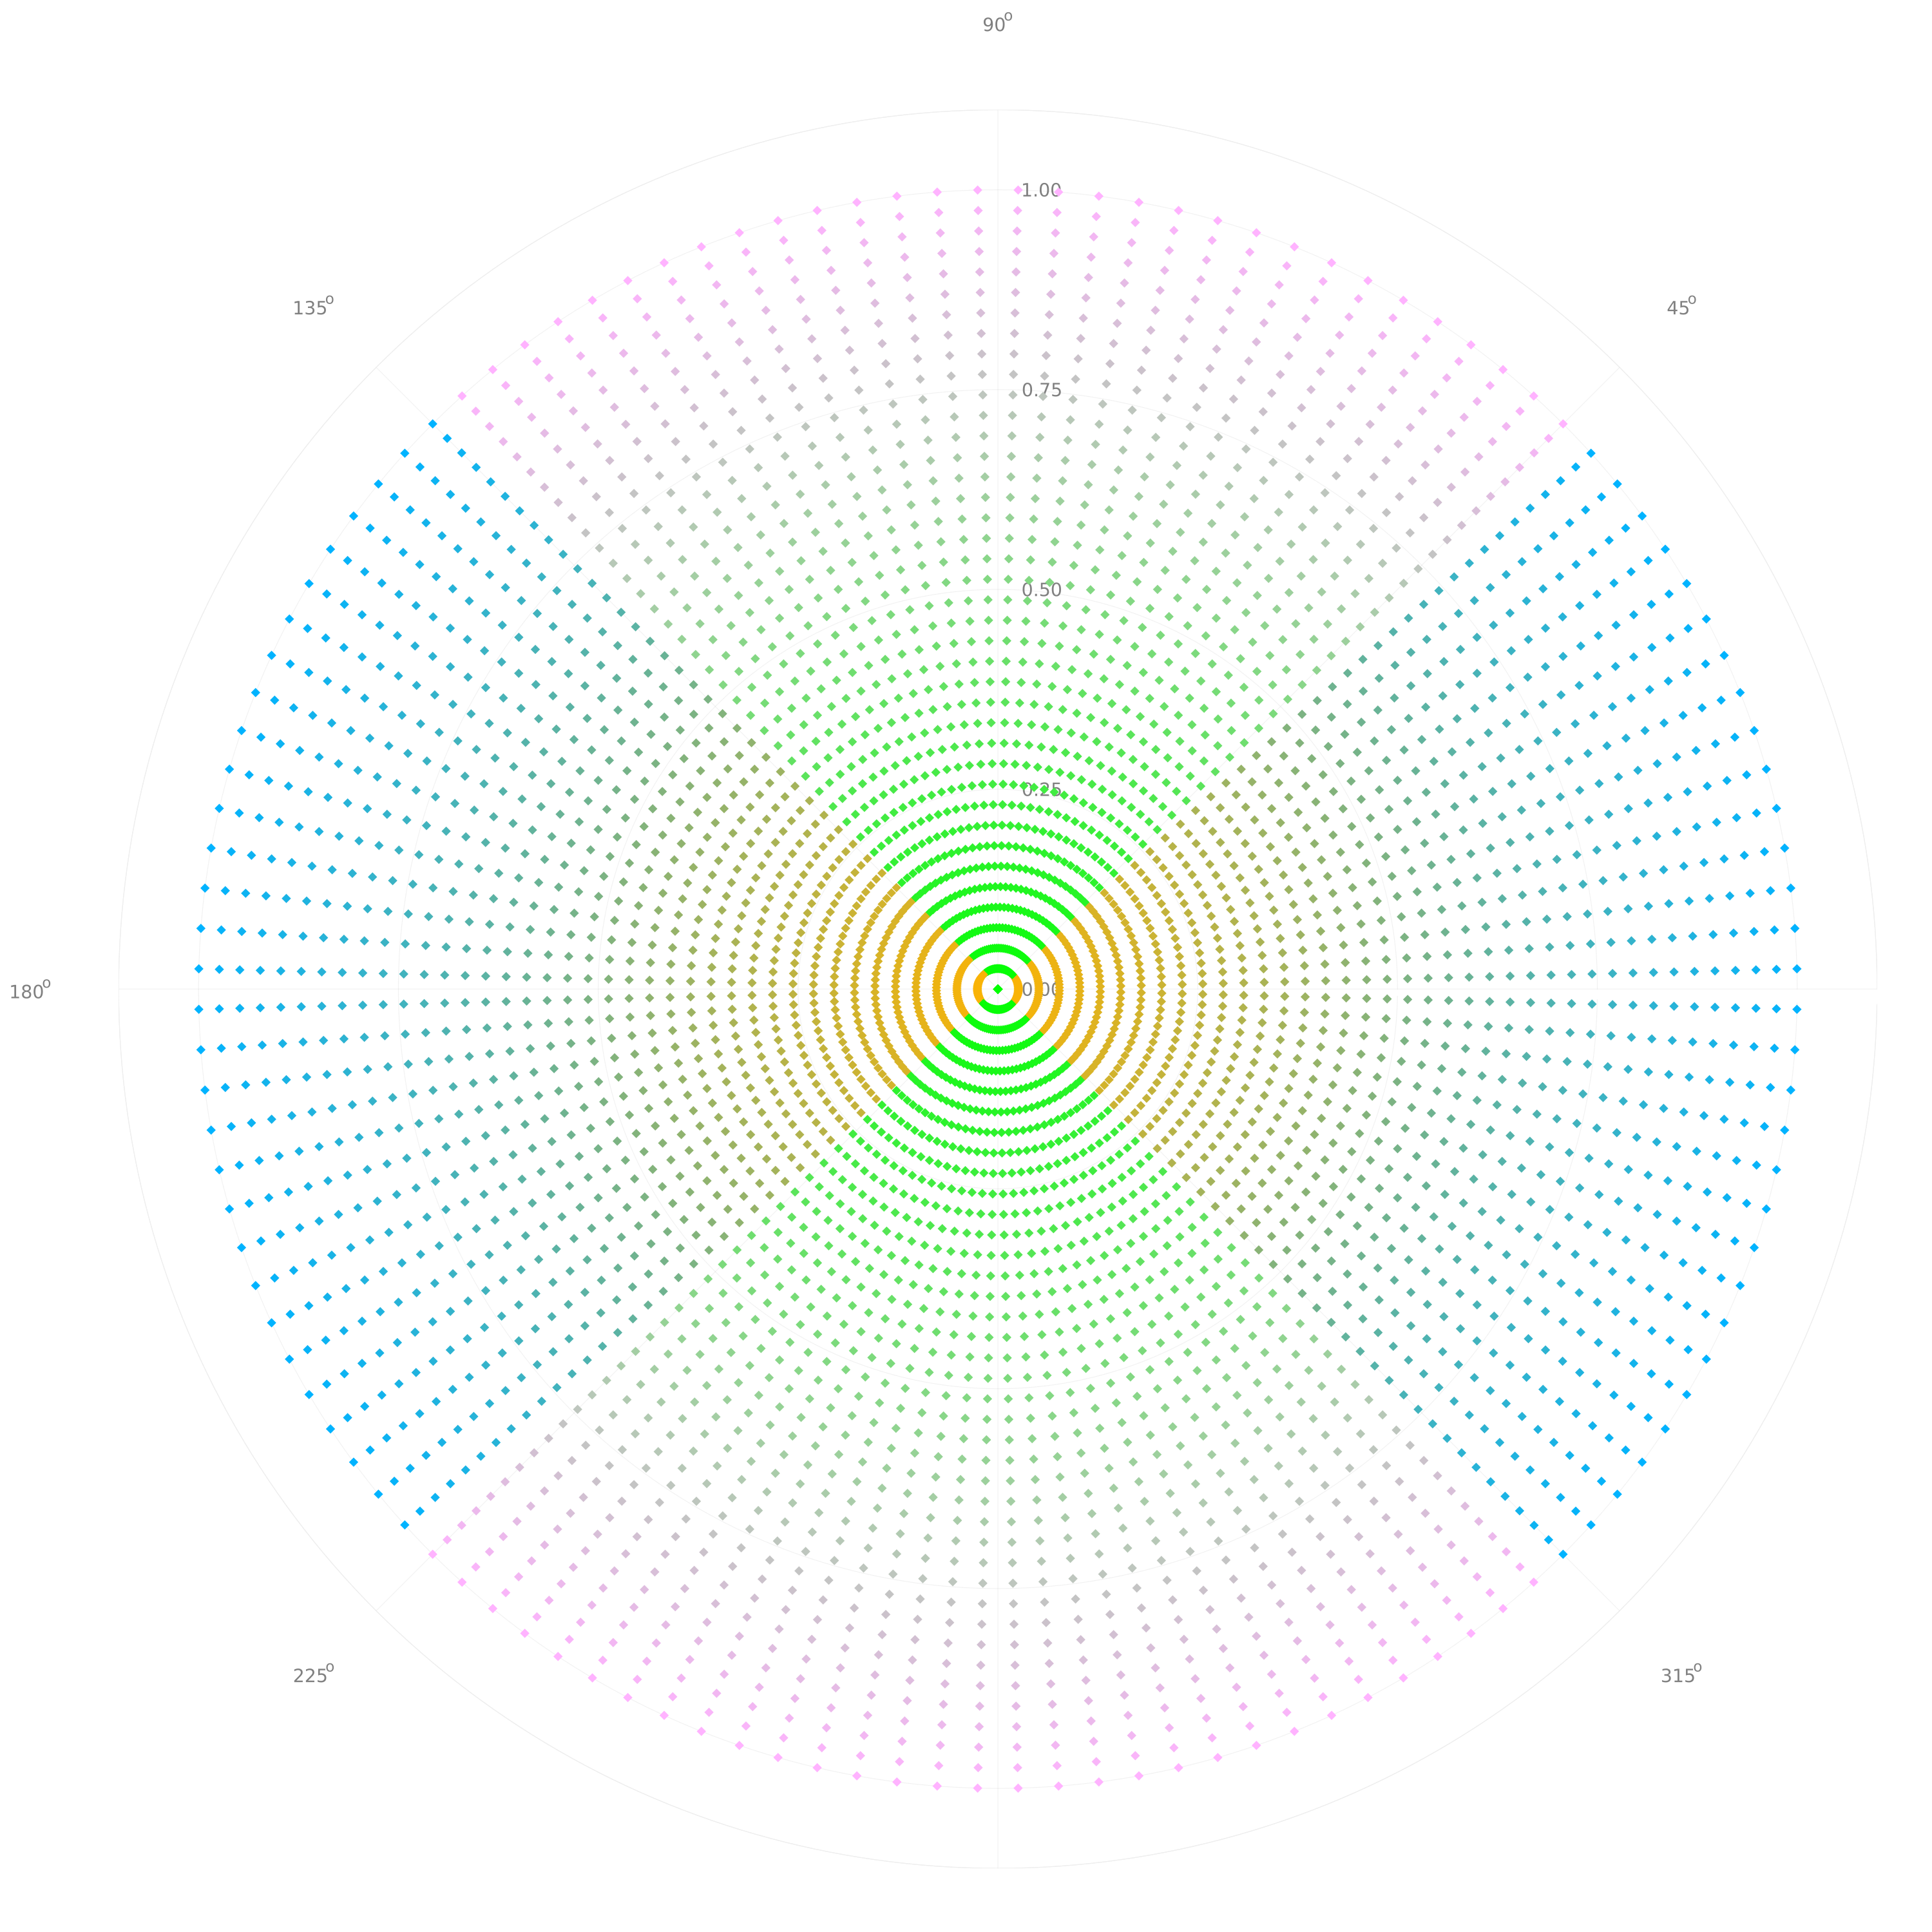
\includegraphics[width=0.3\textwidth]{Figures/targetPlotUnweightedDots.png}}}
    \quad
    \subfloat[\centering]{\makebox[0.45\textwidth][c]{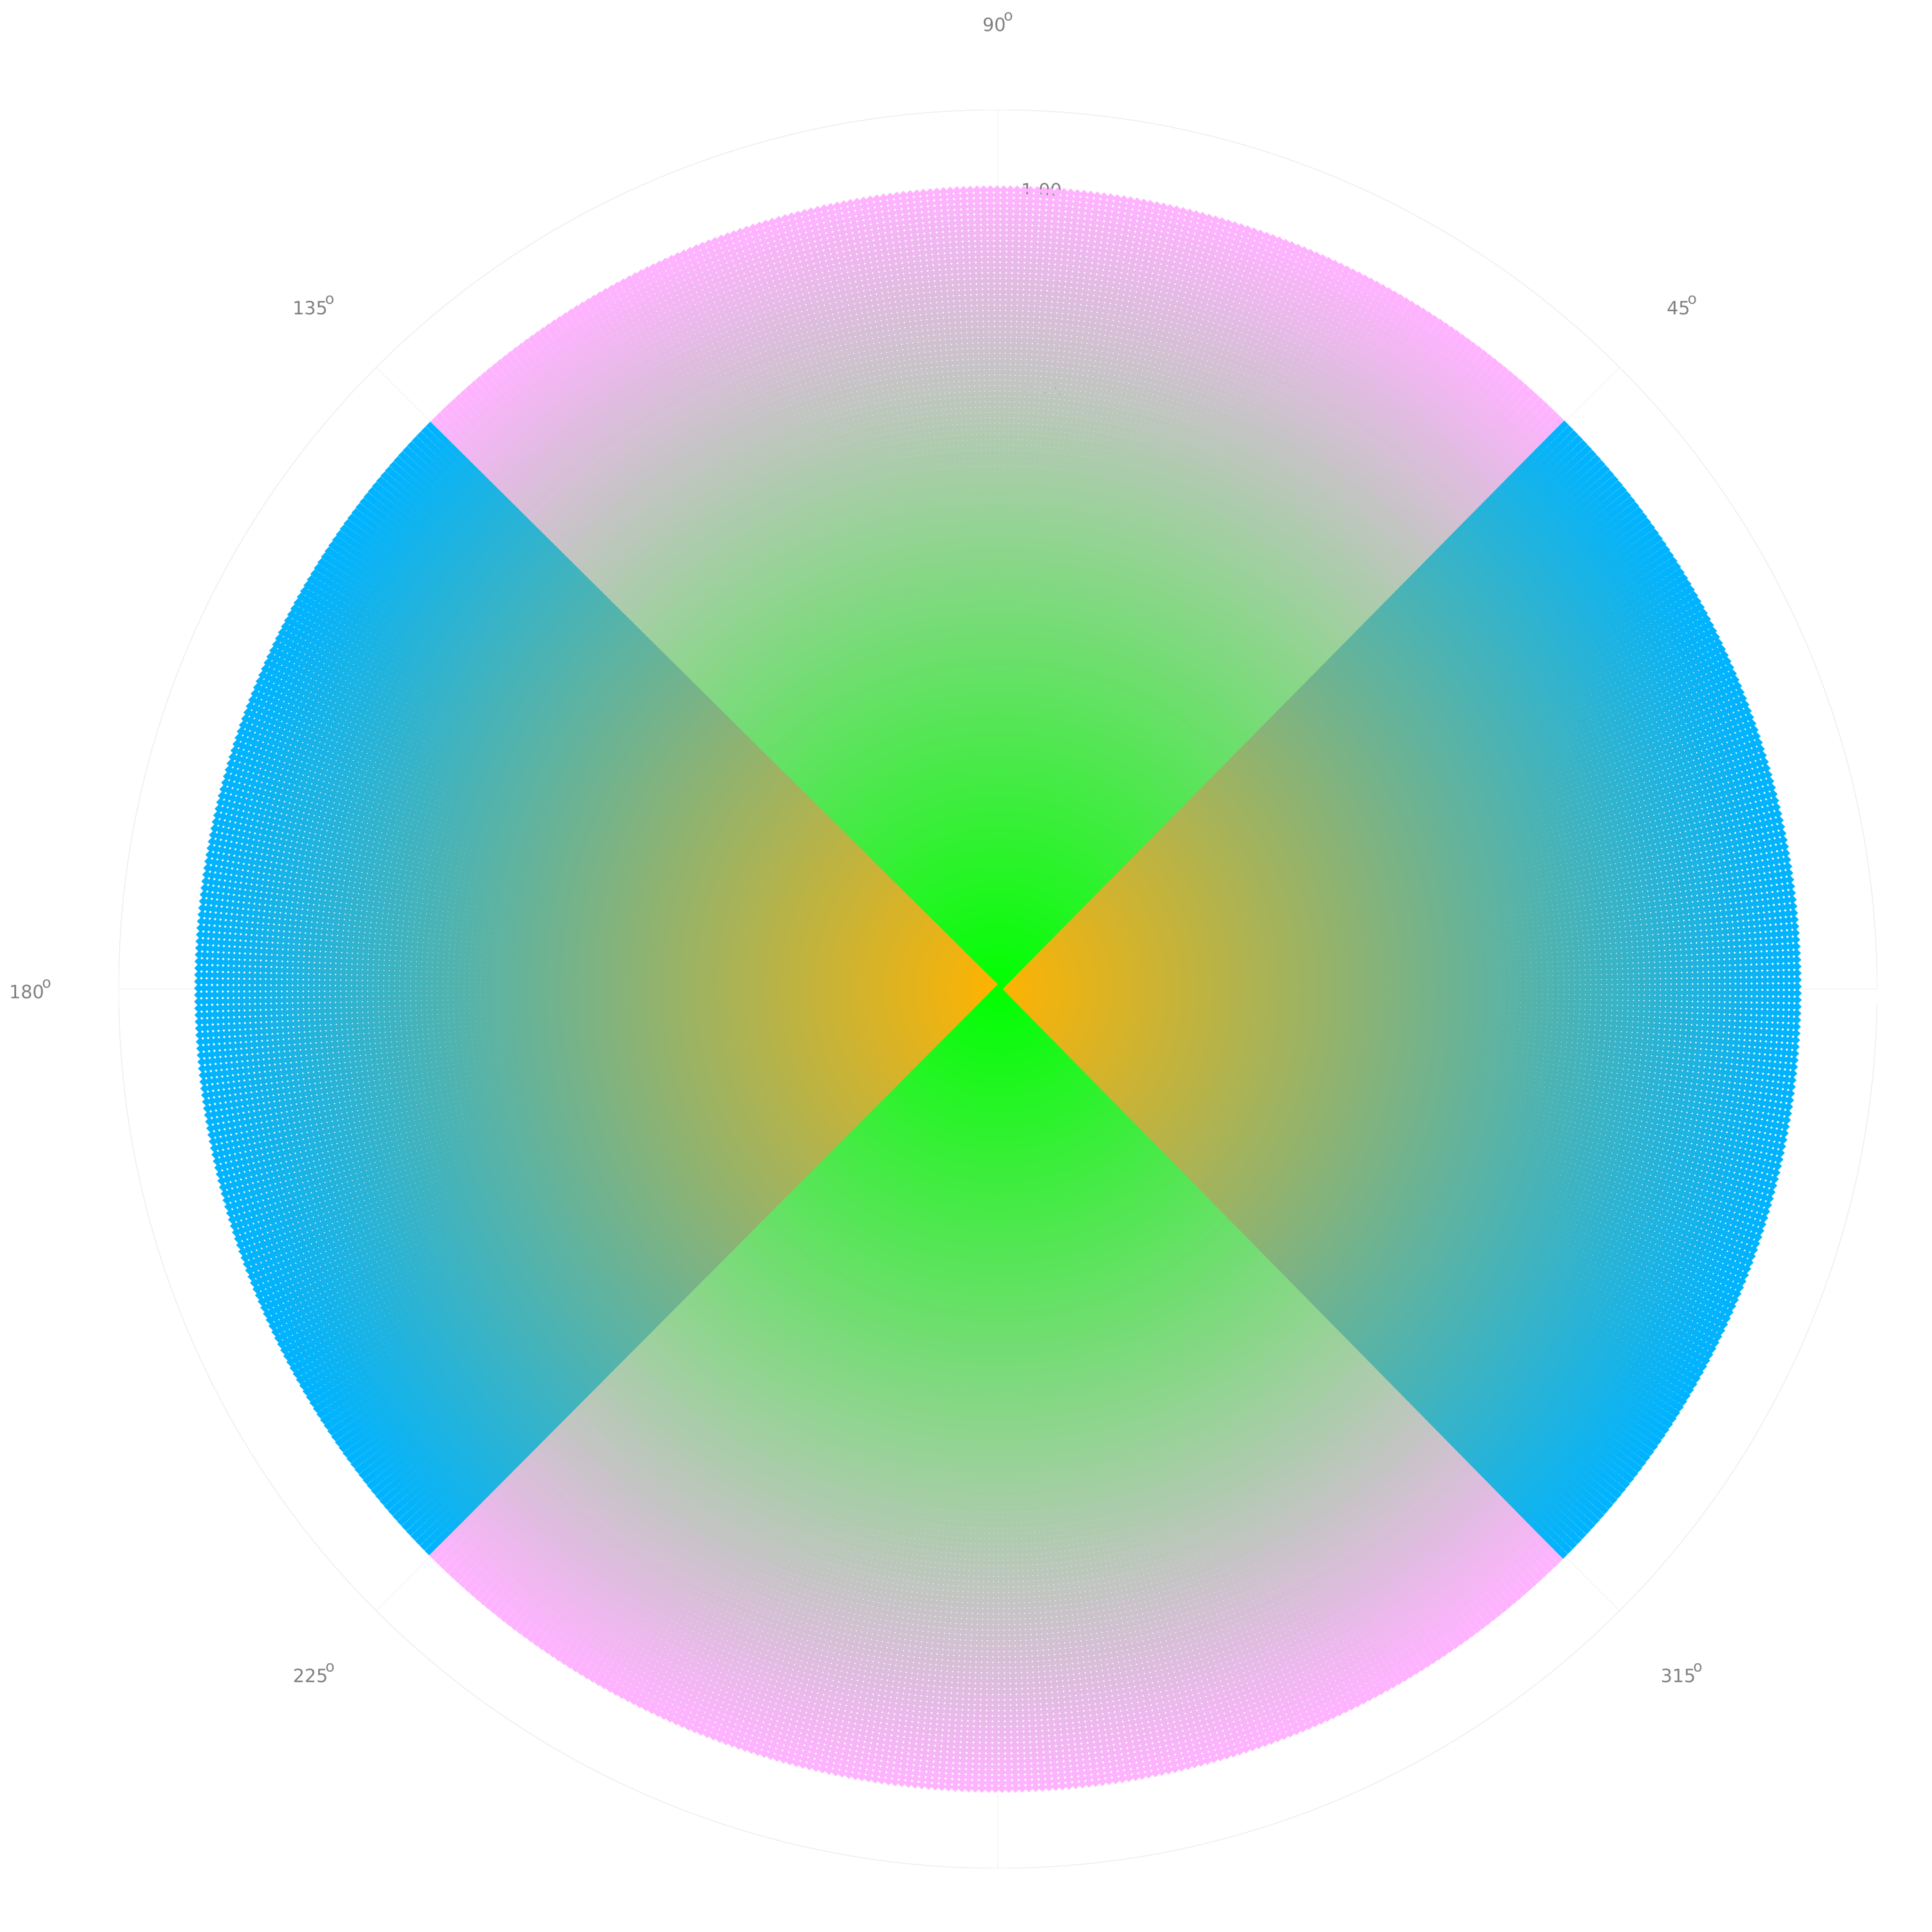
\includegraphics[width=0.3\textwidth]{Figures/targetPlotUnweighted.png}}}
    \centering
    \caption{Nearest radius with no weighting as given by Equation~\eqref{eq:nearest-naive}. The cost function is evaluated to determine a `nearness' value for each point in the polar plot. A perfect radial gradient is observed.}
    \label{fig:nearest-unweighted-vis}
\end{figure}


The first weighted cost function investigated was a simple product of the target's radius $r_\text{t}$ by the difference $\left\lvert \theta_\text{s} - \theta_\text{t} \right\rvert$ between its angle $\theta_\text{t}$ and the search angle $\theta_\text{s}$, normalised with respect to the maximum deviation $\theta_\text{d}$, where
\begin{samepage}
    \begin{align}
        w_\text{simple}(r, \theta) & = \frac{\left\lvert \theta_\text{s} - \theta \right\rvert}{\theta_\text{d}} \label{eq:nearest-simple} \\[0.75em]
        c(r, \theta)               & = \begin{cases}
                                           r \cdot w(r, \theta) & \left\lvert \theta_\text{s} - \theta \right\rvert \leq \theta_\text{d} \\
                                           \infty               & \text{otherwise}
                                       \end{cases}
    \end{align}
\end{samepage}

The intuition for the weighting function given by Equation~\eqref{eq:nearest-simple} is that targets which fall nearer to the search angle are multiplied by a smaller factor and hence considered `nearer'.
This cost function is visualised in Figure~\ref{fig:nearest-simple-vis}.
This simple weighted function was found to be equally unsuitable, as it gave unfair preference to even the radially farthermost target, provided only that it lay close to the search angle such that $\theta_\text{t} \approx \theta_\text{s}$.
An example is provided in Figure~\ref{fig:nearest-weighted-simple}, demonstrating that algorithm pounces straight from target 2 to target 3, skipping over targets 4 and 5.

An offset $C$ was then applied to the multiplicative factor $w(r, \theta)$ to break the property of homogeneity, and hence linearity, of the cost function.
\begin{equation}
    w_\text{non-linear}(r, \theta) = \frac{\left\lvert \theta_\text{s} - \theta \right\rvert}{\theta_\text{d}} + C
    \label{eq:nearest-non-linear-damping}
\end{equation}
This offset was found to behave as a damping term; a control knob that could be leveraged to moderate the influence of angle deviation towards the computed `nearness' of a target position.
This algorithm was observed to behave increasingly like the unweighted `nearest radius' algorithm in Equation~\eqref{eq:nearest-naive} as $C \to \infty$, which is understood through the underpinning theory behind non-homogenous functions.

It was realised through this observation that the `damping term' $C$ behaves in effect like the reciprocal of a directivity constant $D$, where Equation~\eqref{eq:nearest-non-linear-damping} can be re-written as
\begin{equation}
    w_\text{non-linear}(r, \theta) = \frac{\left\lvert \theta_\text{s} - \theta \right\rvert}{\theta_\text{d}} + \frac{1}{D}
    \label{eq:nearest-non-linear-directivity}
\end{equation}
such that $c_\text{non-linear}(r, \theta)$ approximates the unweighted `nearest radius' algorithm as $D \to 0$.
A higher directivity value corresponds to a narrower, more focussed search that prioritising targets that are closely aligned with the search angle $\theta_\text{s}$.
Conversely, a lower directivity value results in a broader, more omnidirectional search, considering targets across a wider range of angles.
Visualisation for this behaviour is provided in Figure~\ref{fig:nearest-directivity-2-vis} and in Appendix~\ref{apx:nearest-target-directivity}.
\begin{figure}[hbtp]
    \subfloat[\centering Nearest radius multiplied by angle deviation as given by Equation~\eqref{eq:nearest-simple}. Great emphasis is seen for points along each search angle. \label{fig:nearest-simple-vis}]{\makebox[0.45\textwidth][c]{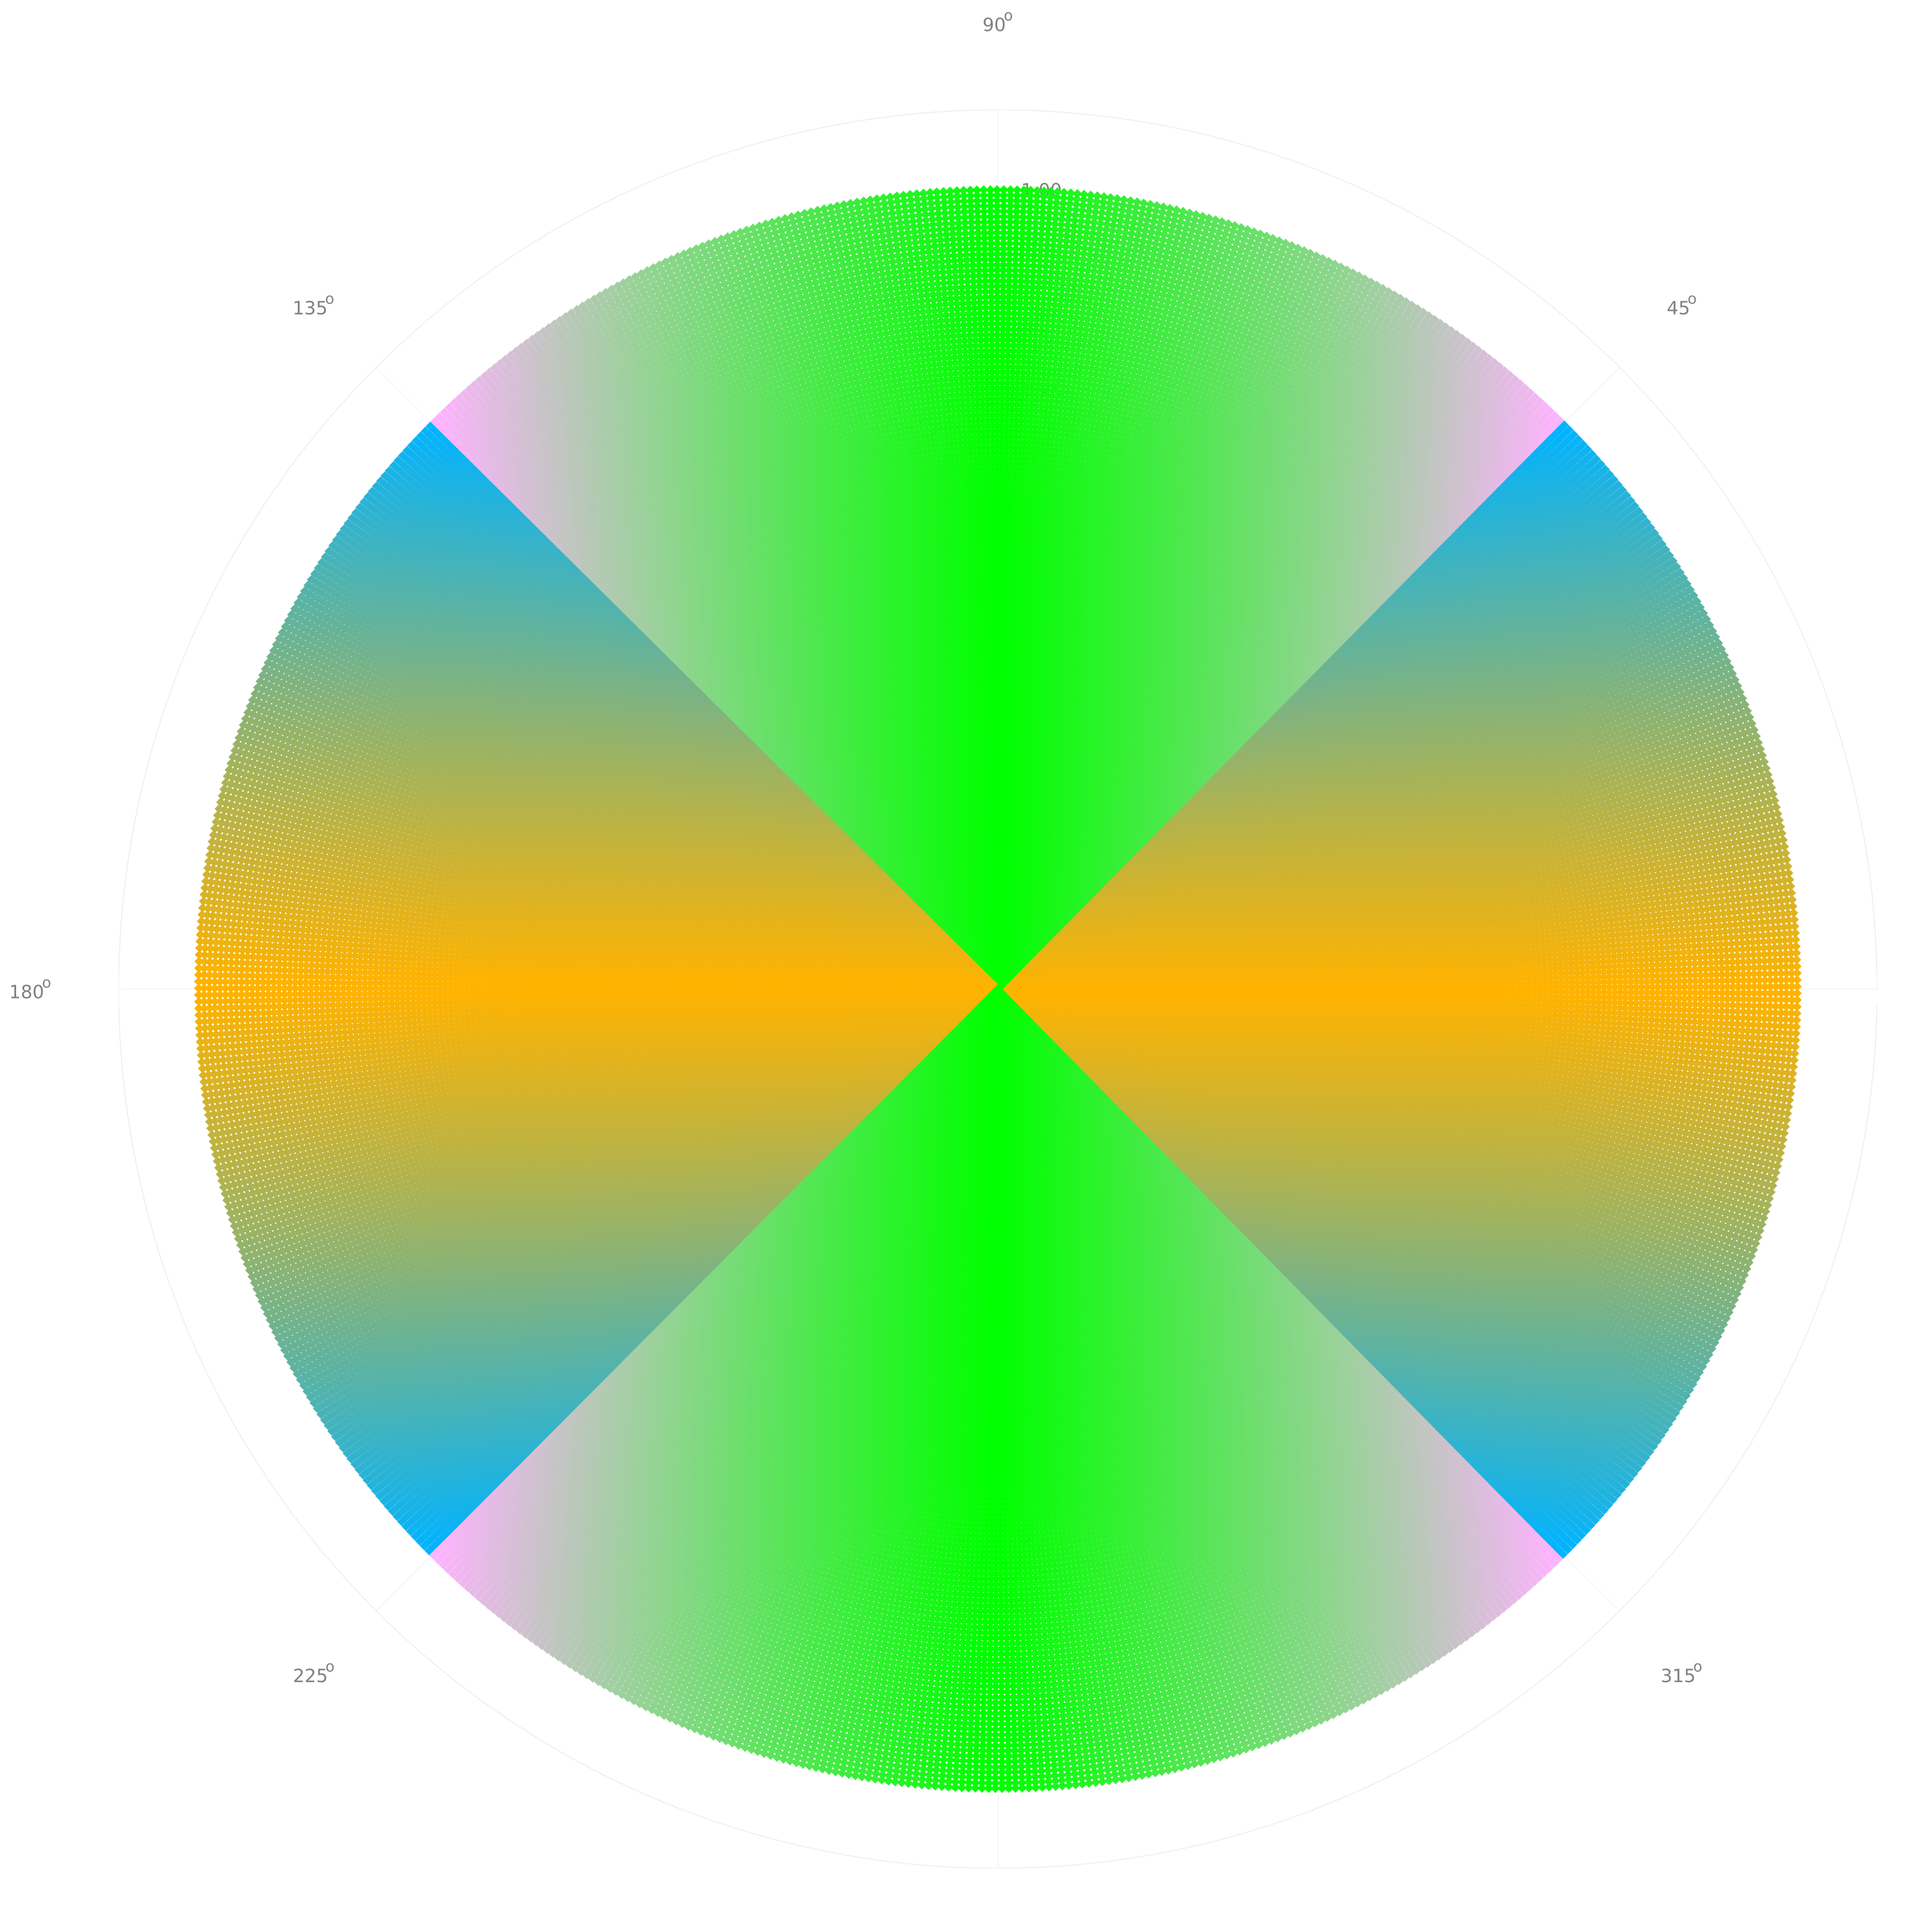
\includegraphics[width=0.3\textwidth]{Figures/targetPlotWeightedSimple.png}}}
    \quad
    \subfloat[\centering Non-linear weighting as given by Equation~\eqref{eq:nearest-non-linear-directivity} with directivity $D = 2$. \label{fig:nearest-directivity-2-vis}]{\makebox[0.45\textwidth][c]{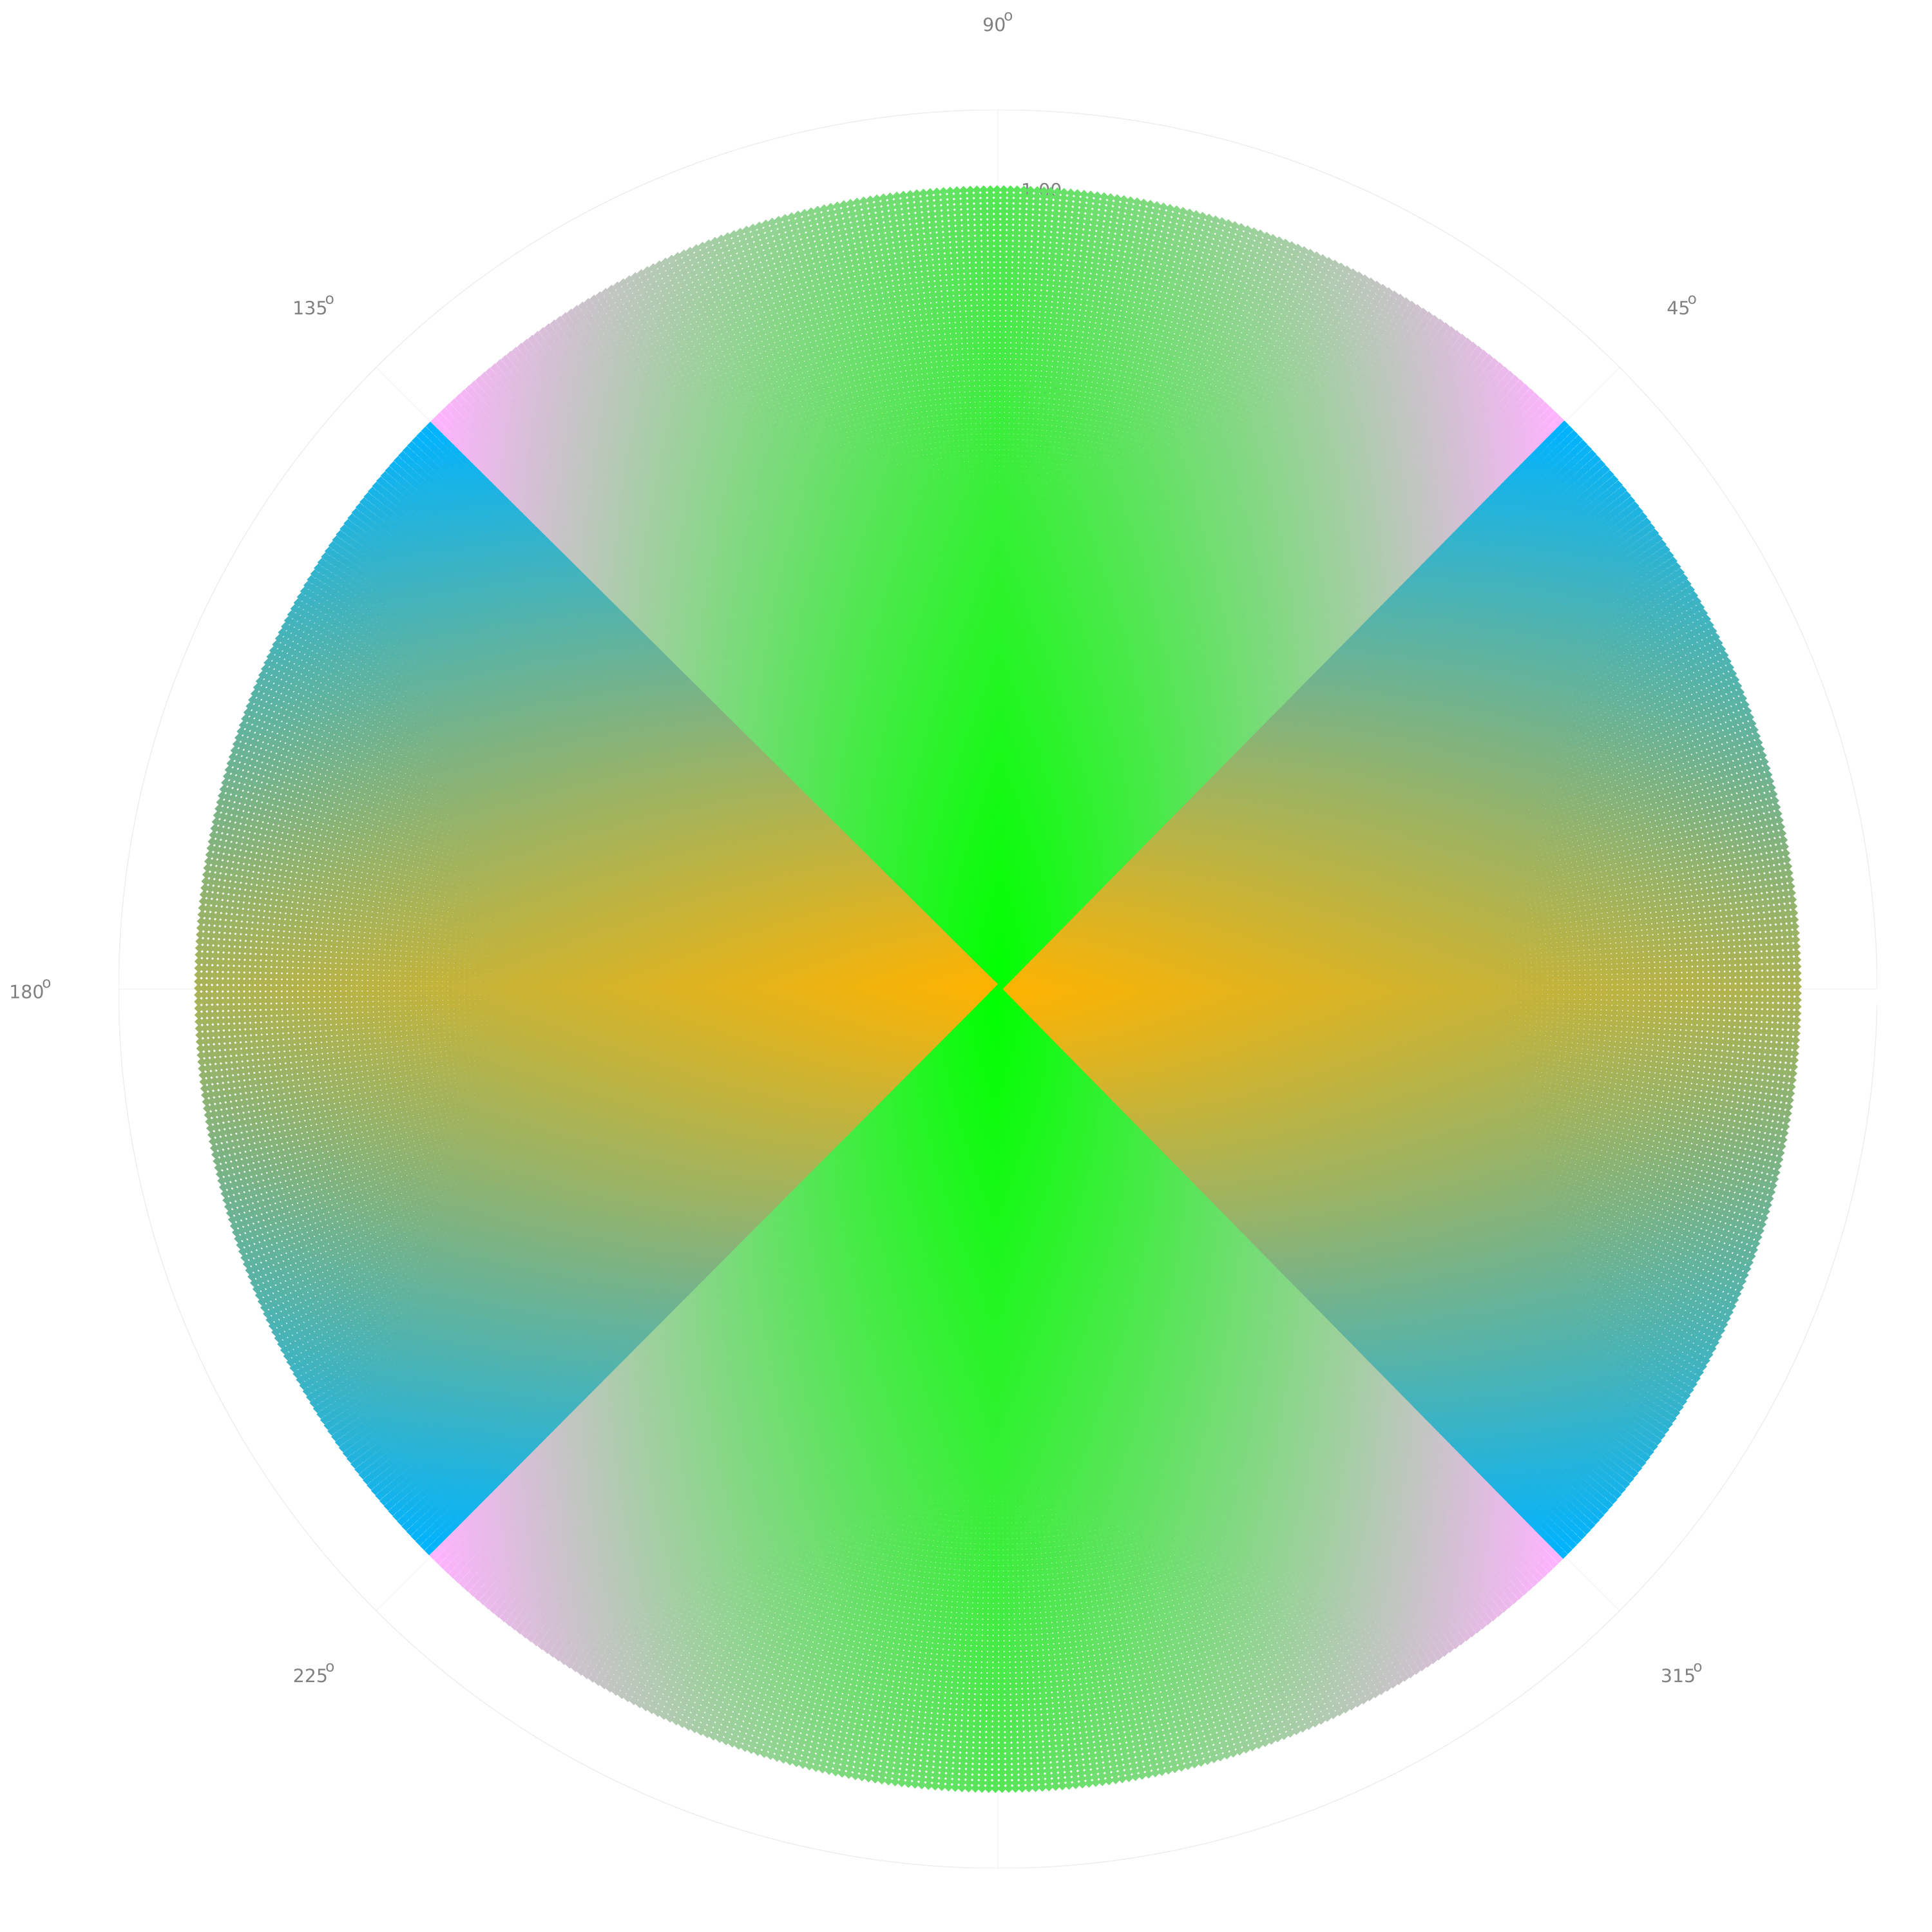
\includegraphics[width=0.3\textwidth]{Figures/targetPlotWeightedNonLinear2.png}}}
    \centering
    \caption{Weighted cost function visualisations.}
\end{figure}

Following implementation of this non-linear cost function, empirical testing found that the weighted nearest-target algorithm as given by Equation~\eqref{eq:nearest-non-linear-directivity} indeed felt significantly more natural and intuitive.
Examples are provided in Figure~\ref{fig:nearest-directivity-1} and Figure~\ref{fig:nearest-directivity-2} below, where it was found that the same input sequences as presented in Figure~\ref{fig:nearest-unweighted-1} and Figure~\ref{fig:nearest-unweighted-2} produced the expected `intuitive' results when using Equation~\eqref{eq:nearest-non-linear-directivity}.

A concern in the design of the algorithm was ensuring the reliability of the navigation scheme.
Specifically, it was important to avoid `dead zones' where certain pad locations might become unreachable due to their relative angular position.
It is observed that the non-linear function as weighted by Equation~\eqref{eq:nearest-non-linear-directivity} does not guarantee that every target position is reachable, due to its dependency on angular deviation.
Although a formal proof of the algorithm's reliability was not conducted, it was deemed acceptable to assume a sufficiently dense distribution of pads on the \ac{PCB}.
In such cases, even if a particular pad is not directly accessible due to its angular position, it should still be reachable by a sequence of intermediate pounces through other pads.
This assumption relies on the density of pad locations on typical \acp{PCB}, where multiple paths often exist to reach a specific target.
An example of this is provided in Appendix~\ref{apx:nearest-target-unreachable}.

It was noticed that the directivity constant $D$, which determines the influence of angular deviation, could be a subjective parameter.
Similar to varying preferences for mouse tracking speed \cite{9893626}, the ideal directivity constant may vary between operators.
A natural directivity constant for one operator may feel too `narrow' or too `broad' for another.
A mechanism for the operator to adjust the directivity constant was thus proposed.
This could be implemented in the interface as a slider, allowing the operator to fine-tune the algorithm's behaviour to match their preferences.
To promote understanding of the parameter's impact, a a polar pattern diagram or other visual could be displayed alongside.

An alternative approach to controlling angular `focus' was proposed by increasing the number of search sectors $N$.
Rather than searching the four cardinal directions, the usage of six or eight search sectors was considered to provide more precise target selection by reducing the maximum allowed deviation $\theta_\text{d}$ from the search angle $\theta_\text{s}$ for each search sector.
This approach would require additional keys, such as the QE and/or ZXC keys on a standard QWERTY-layout keyboard or the keys on a numeric keypad.
An alternative implementation could use a modifier key that temporarily rotates the set of search angles by \qty{45}{\degree}, providing more efficient navigation to diagonal targets using the WASD keys.


\subsubsection{Mouse Navigation}

Upon testing the pouncing scheme as in Figure~\ref{fig:nearest-target-interface}, a realisation was made that keyboards are fundamentally unsuitable for precise positioning and spatial control.
It was found that navigation to a specific target with discrete inputs became increasingly cumbersome as the number of pads increased, requiring many intermediate jumps to reach the desired location.
The obvious realisation was made that the continuous nature of mouse input made it a more suitable solution for precise and efficient spatial input, even with discrete targets.
It was realised that inspiration from \texttt{vim}-style editors was misguided, as inputs to a \ac{PnP} are spatial, not textual.
Keyboard navigation in \texttt{vim} is highly efficient as the user's hands must be on the keyboard to type \cite{10.31510/infa.v17i2.1066}.
Although some key input may exist for the \ac{PnP} machine, the primary task is spatial navigation --- and this is best achieved through a mouse.

Keyboard-based pouncing may be viable if used with \ac{CV} routines that identify one centroid per component instead.
Viability may also be realised by pouncing only to component pads that match the footprint of the picked component, considerably reducing intermediate pounces.
However, both approaches require \ac{CV} routines that are considerably tougher to implement.
These options may be interesting to investigate further as future work, but a decision was made not to pursue them further.

Adopting a mouse as the primary input method expands the set of potential locations to again include all points, assuming sufficiently high camera resolution.
To simplify this interaction and maintain the precision and efficiency of the pouncing approach, a pad-expansion scheme is proposed.
Each region in the diagram is associated with a unique site, and every point within a region is closer to its corresponding site than to any other site \cite{10024454}.
A Voronoi diagram as shown in Appendix~\ref{apx:voronoi} is a geometric construct that divides a space into regions based on proximity to a set of points, called `sites'.
In the context of the \ac{PnP} machine, the identified pad centroids can be treated as sites, and a Voronoi decomposition can be utilised to partition the image into regions surrounding each pad.

By implementing a Voronoi partition in the user interface, each mouse click can be associated with the nearest identified pad location, regardless of the precise position of the click within the corresponding Voronoi region.
This pad-expansion eliminates the need for pixel-perfect accuracy from the operator to precisely target a centroid.
This combination of mouse input and intelligent interpretation should enable both precise control and efficient navigation, reducing cognitive load and promoting a state of flow.

\subsubsection{Heads-Up Display}

As discussed in Section~\ref{sec:User-Interface-Technical}, the \ac{HUD} is implemented as an \ac{HTML} \texttt{<div>} element that sits atop the received video feed.
This \ac{HUD} is responsible for communicating machine state to the operator to enhance their sense of control.
A large instruction bar is displayed at the top of the \ac{HUD} to inform the operator as to the currently expected action, and toast-style notifications are used for event and error reporting.
A state indicator bar displaying information about the mechanical condition of the \ac{PnP} machine is shown at the bottom of the \ac{HUD}.
An example of the developed \ac{HUD} is shown in Figure~\ref{fig:component-placed}.
\begin{figure}[hbtp]
    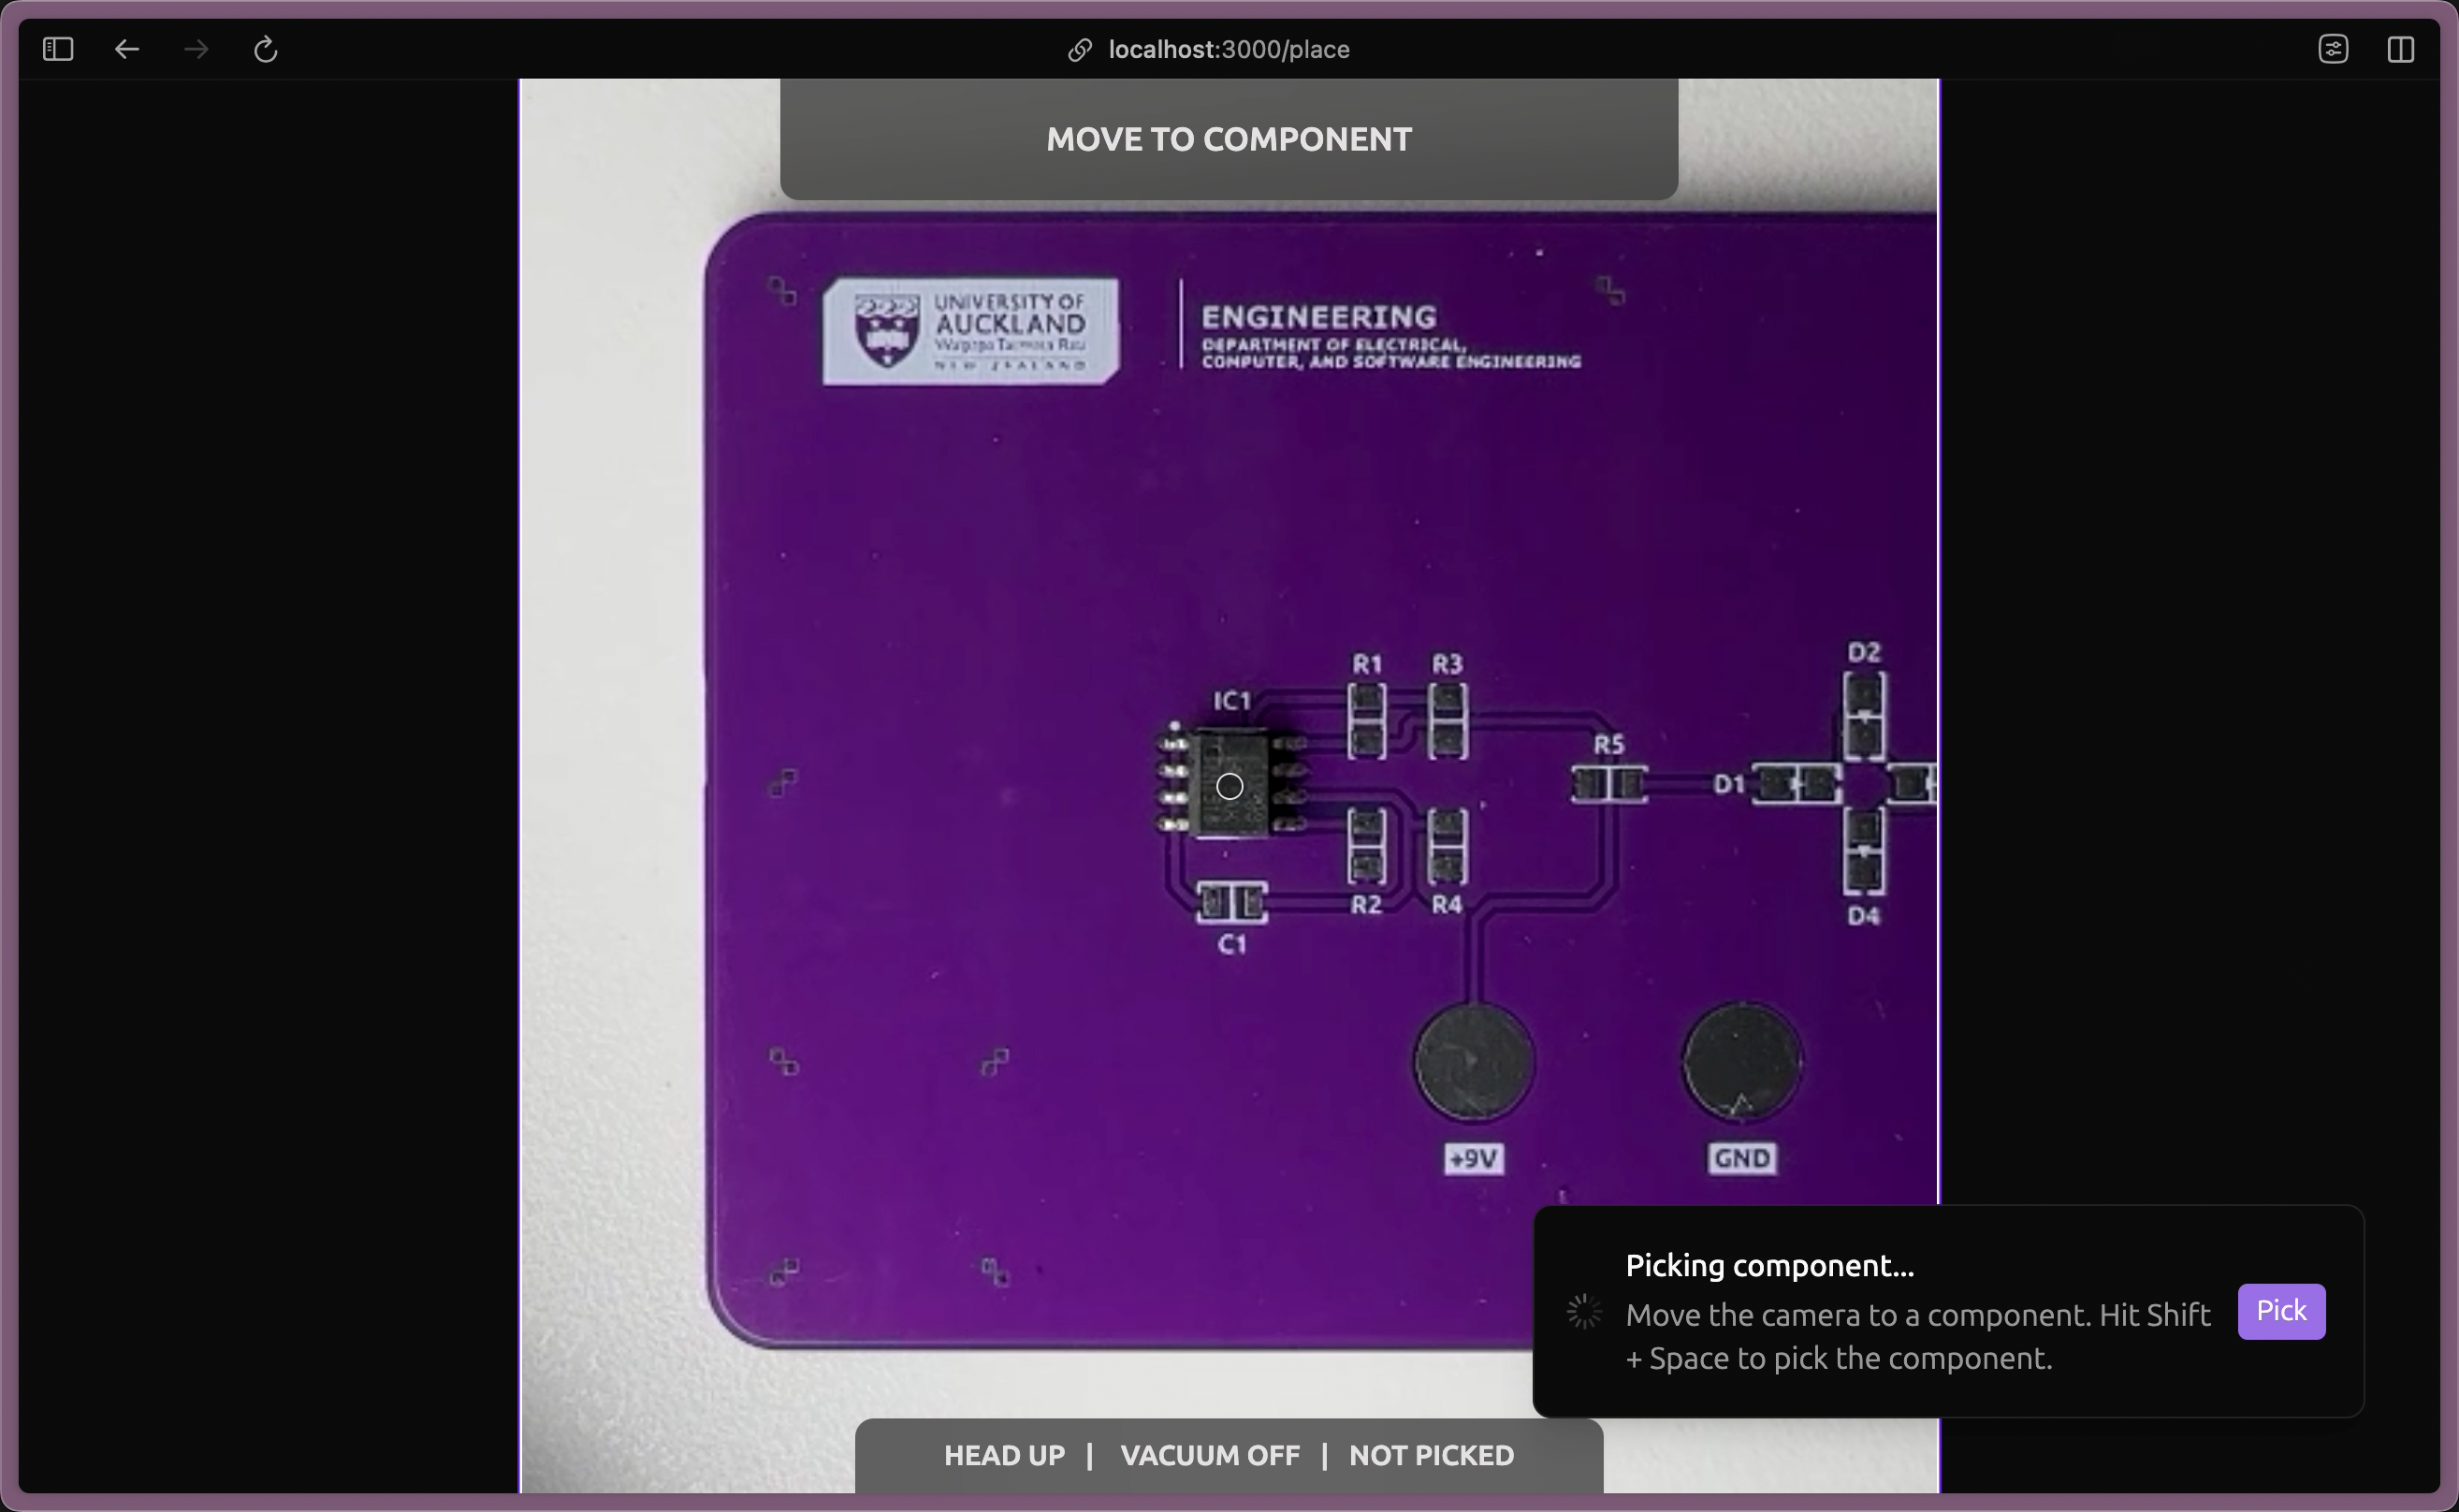
\includegraphics[width=0.8\textwidth]{Figures/component-placed.png}
    \centering
    \caption{Screenshot of \acf{HUD} after a successful component placement. Target markers are not shown.}
    \label{fig:component-placed}
\end{figure}

In addition to these elements, the \ac{HUD} additionally comprises of four other indicator types:
\begin{enumerate}
    \item a cursor crosshair.
          This is discussed in Section~\ref{sec:User-Interface-Technical}, and is a \ac{CSS} style applied to the mouse pointer within the \ac{HUD} overlay element.
    \item a nozzle centre indicator.
          This is a grey circle fixed to the position of the vacuum nozzle when in the `upward' position, as shown in Figure~\ref{fig:head-up}.
          This indicator is used to communicate the origin $(0, 0)$ of the machine to the operator.
    \item a selected target indicator.
          This is a temporary purple circle that indicates the currently selected target marker for the gantry to next translate to.
          When mouse input is presented, this indicator is used to mark the clicked coordinates.
          As in Section~\ref{sec:Controller-Interface}, the machine controller will respond to the interface with a \texttt{MOVED\_DELTAS} handshaking message upon successful gantry translation, which is acknowledged by the interface by translating this purple indicator to the nozzle centre position.
    \item target markers.
          These are grey squares drawn atop any centroids of interest as identified by the \ac{CV} routines.
          These centroid positions are transmitted to the interface by the \texttt{TARGET\_POSITIONS} \ac{protobuf} message, and are used as the `pounce' targets for the nearest-target algorithm discussed in Section~\ref{sec:Nearest-Target}.
\end{enumerate}

As discussed in Section~\ref{sec:Nearest-Target}, consideration was made towards implementing a set of slider controls for the operator to fine-tune such runtime configurations as the directivity constant $D$ or fixed `nudge' distance on-the-fly.
This could be achieved either directly in the \ac{HUD}, or potentially as a sliding sidebar window.
This proposal was de-prioritised following the shift to mouse input, but should be considered for future work.

Another discarded proposal to enhance the \ac{HUD} for pouncing was the implementation of radial `guide' lines that visually demarcate each individual search sector.
It was expected that this would prevent ambiguity for targets that lie along a search sector boundary.
Another potential solution requiring further investigation could be the introduction of overlap between search sectors, such that two pounce directions could select such targets.


\subsubsection{Recommendations for Future Enhancements}\label{sec:Future-Enhancements}

Several enhancements to the user interface have been identified, through which user studies can be performed to profile improvement over the current implementation.

\paragraph{Input Scheme}

A proposed method to improve navigation efficiency is the use of number keys to enable rapid access to predefined locations on the machine bed.
The operator could use the number keys (`1', `2', `3', etc.) to instantaneously `jump' to hard-coded parts bin positions, streamlining the process of selecting and picking up components.
This functionality could be further expanded to support operator-programmable saved positions, allowing for efficient access to frequently used locations on the machine bed.
This customisable navigation feature is expected to significantly reduce the time required to move the placement head between locations of interest, enhancing the overall efficiency and usability of the real-time system.

A click-and-drag rotation feature could be added, allowing the operator to rotate the picked component by clicking and dragging the mouse cursor in a circular motion.
It is hypothesised that this would provide a more intuitive and interactive method for adjusting the component's rotation than the current keyboard-based input scheme.

\paragraph{Contextual Awareness}

A potential area for future improvement lies in addressing the `desert fog' problem identified in the literature on \acfp{ZUI} \cite{10.1145/288392.288578}.
It is expected that providing the operator with contextual awareness of their current location within the larger workspace could enhance navigation efficiency and reduce cognitive load.

One approach to mitigating this `desert fog' is the addition of a minimap indicator to the user interface \cite{10.1145/586081.586086}.
This minimap would display a scaled-down overview of the entire \ac{PCB}, with a highlighted region indicating the operator's current \ac{FoV} within the zoomed-in video feed.
This would provide the operator with a constant visual reference of their location within the larger context of the board, allowing them to easily orient themselves and navigate to desired areas of the \ac{PCB}.
The minimap could also be made interactive, allowing the operator to click on a specific location on the minimap to instantly jump to that region in the zoomed-in view to further enhance navigation efficiency.

Another potential direction for future work is the implementation of adjustable machine zoom scales.
Similar to the adjustable `Snap Grid' functionality in Altium Designer \cite{altiumChooseSnap}, the zoom scale would dictate the precision of inputs to provide the operator with control over the granularity of movement and placement.
This could be implemented as a multi-layered interface, inspired by research into \Acp{ZUI}, with three distinct layers of interaction that offer varying levels of precision as detailed in Appendix~\ref{apx:multi-layer-interface}.
The multiple precision scales and varying zoom levels of this multi-layered interface is expected to provide a natural and efficient solution for navigating the placement head around the \ac{PCB}.

\paragraph{Feed-Forward Control}

The use of feed-forward control with still images was considered as a way to mitigate the limitations of real-time video streaming latency.
This approach would involve sending a sequence of still images, or a very low frame-rate video, to the user interface.
The interface would then use a predictive model \cite{Dragan2013} to extrapolate the machine's movements between the received images, creating a smooth and responsive visual experience for the operator.
This method, while relying heavily on the accuracy of the predictive model, could potentially overcome the limitations of real-time video streaming --- particularly when dealing with slow or inconsistent network connections.


\section{Discussion}\label{sec:Discussion}
% ? This is where you discuss and analyse the results you reported in the previous section
% ? Explain what you have found and what it means
% ? Use statistics, proper graphs, and tables to argue and validate your results
% ? Benchmarks and comparative study
% ? Research limitations
% ? Discuss how the research questions are answered and objectives are met

% * Research approach
% A gap is identified in numerically-controlled machine tools that are deliberately driven in real-time with active assistance; a hybrid tool that supplements a human's affinity for big-picture understanding with the precision of an electromechanical machine.
% Such a machine is neither fully-automated nor fully-manual, and requires investigation into the necessary design and usability considerations for intuitive use.
% This research aims to identify and understand these considerations to develop a functional prototype of such a real-time \ac{PnP} machine.
% It is hypothesised that such a machine will require some aspect of active alignment assistance to be useful, but development will initially target an open-loop machine with sufficient responsiveness and accuracy for closed-loop active assistance.

% This research will consequently investigate the integration of light \ac{CV} with a traditional $x$-$y$ gantry and vacuum head to assist a human operator with \ac{SMT} component placement and alignment atop a \ac{PCB}.
% To achieve intuitive real-time control, significant scope is also foreseen for the research and development of an accompanying user interface that minimises cognitive load and promotes a state of flow

% It is proposed that \ac{CV} `feedback' can be introduced to this open-loop control path to achieve enhanced machine performance.
% This \ac{CV} would provide active alignment assistance to the human operator, offloading the burden of fine positioning to the machine.
% In such an operating profile, the operator would be solely responsible for rough position identification.
% Once component leads have been roughly associated with its corresponding component pads, active alignment assistance would correct any rotational error and perform final `wicking' of the component into place.

The prototype machine successfully picks and places components, demonstrating the viability of the core concept.
However, achieving a high degree of accuracy and a user experience conducive to flow proved challenging.
The initial aim of real-time shared control, where the machine responds organically to continuous operator input, was not fully realised.
This was primarily due to limitations of the machine's mechanical speed and responsiveness, and the subsequent impact on the operator's ability to maintain a state of flow.

This research highlighted the importance of a robust and low-latency communication protocol for real-time control.
The \ac{WebRTC} protocol, with its demonstrated latency of \qty{130}{\milli\second}, emerged as a viable solution for streaming real-time video.
This low latency, combined with the efficient data exchange facilitated by WebSockets and \Aclp{protobuf}, ensured responsive communication between the user interface and the machine controller.

The user interface, critical for a seamless user experience, underwent several iterations.
The initial exploration of a joystick-based input scheme with shared control, inspired by video game interfaces, was ultimately abandoned.
The lack of a clearly defined center point on the joystick hindered precise control.
This decision, although justified, restricted the system's ability to achieve the envisioned fluid human-machine interplay.
The subsequent adoption of a keyboard-based pouncing mechanism, initially promising, also revealed limitations.
The discrete nature of keyboard input proved less effective for spatial navigation, particularly for \acp{PCB} with a high density of target pads.
This led to the adoption of a mouse as the primary input method.

Empirical evaluation of the nearest-target algorithm led to the development of a weighted cost function that considers both radial distance and angular deviation.
This produced an intuitive and predictable pouncing behaviour.
However, the subjective nature of the directivity constant was identified, as user preferences for this parameter could vary, suggesting the need for a configurable directivity setting in future iterations.

The developed \ac{CV} routines played a crucial role in enabling assisted component placement.
The implemented centroid-finding algorithm demonstrated a high degree of accuracy in identifying component pad locations, providing the foundation for the pouncing navigation scheme and proposed implementation of closed-loop control for component wicking.
Further research into advanced \ac{CV} techniques, such as component recognition and solder paste detection, could significantly enhance the prototype's capabilities and automation level.

This project highlighted the challenges of balancing speed and accuracy in a real-time system.
While low-latency video streaming and message passing were achieved, the responsiveness of the mechanical system emerged as a bottleneck.
The prototype's performance suggests that a more sophisticated mechanical design, potentially incorporating higher-quality components and more precise actuation mechanisms, is crucial for achieving the desired level of accuracy and speed in a hybrid machine tool.


\section{Conclusions}\label{sec:Conclusions}
% ? What can you definitely say?
% ? Summaries of your contributions
% ? Future research directions

% ? Do not repeat your abstract
% ? Keep it clear and concise
% ? Emphasise what you consider to be the significant findings or outcomes of the investigation
% ? Refer to your objectives
% ? Should provide technical information summary
% ? Should not contain any new information
% ? Based on your results and analysis, what can you conclude?
% ? You can then summarise your contributions, using a bullet point or numbered listing
% ? Present future directions for your research, to address the limitations you identified

The research successfully demonstrated the feasibility of a real-time, vision-assisted \acl{PnP} machine for rapid prototyping.
The prototype machine revealed key insights into the challenges of integrating real-time control, \acl{CV}, and intuitive user interfaces.

This research brought about several key findings and contributions.
Real-time video streaming with \ac{WebRTC} achieved sufficiently low latency for viable hybrid control.
The combination of WebSockets and \aclp{protobuf} provided efficient real-time data exchange between software modules.
A \ac{CV}-fed nearest-target algorithm improved the intuitiveness of keyboard-based pouncing.
Finally, a mouse, with its continuous input, emerged as a more suitable input device for precise spatial navigation.

Based on the findings, it is concluded that the initial aim of a real-time hybrid \ac{PnP} machine presents a challenging but achievable goal.
However, this requires further research and development, particularly in developing more responsive mechanical systems and refining the \ac{CV} routines for robust component recognition.
Mechanical responsiveness emerged as a constraint on placement accuracy and user interface efficacy, hindering the development of the envisioned fluid human-machine interplay.

The user interface would benefit from additional features to enhance contextual awareness, such as a minimap and adjustable zoom scales.
Additionally, such advanced user interface features as a zoomable interface and feed-forward control could further enhance usability.
Finally, the implementation of closed-loop control with autonomous component wicking could significantly improve overall placement speed and accuracy.

Future research should investigate applying the developed software solutions, including the \ac{CV} routines and user interface, to existing desktop \acl{PnP} machines.
This approach could potentially leverage the precision and speed of these machines whilst introducing real-time control and enhanced user interaction.
Doing so would bring the original vision of a truly intuitive and efficient rapid prototyping tool closer to reality.

This research lays the groundwork for future work in this domain, paving the way for the development of real-time hybrid machine tools that empower engineers to prototype electronic circuits with greater speed and precision.

%% ------------------------------- REFERENCES -------------------------------------------
\bibliographystyle{IEEEtran}
\addcontentsline{toc}{section}{\refname}\bibliography{RefDatabase}

\newpage{}

%% -------------------------------------------------------------------------------------------
%% ----------------------------------- APPENDICES---------------------------------------------
%% -------------------------------------------------------------------------------------------
\input{sections/appendix}
% -------------------------- End of Appendices --------------------------------

\end{document}
%% ---------------------------- END OF DOCUMENT -------------------------------